\documentclass[xcolor=svgnames, t]{beamer}

\usepackage[utf8]{inputenc}
% \usepackage{booktabs, comment}
\usepackage[absolute, overlay]{textpos}
\useoutertheme{infolines} 
% \usepackage{csquotes}
\usepackage{caption}
\usepackage{cancel}
\usepackage{enumerate}
\usepackage[french]{babel}
\usepackage{xcolor}

% biblio management
\usepackage[backend=bibtex,style=authoryear,citestyle=authoryear]{biblatex}
\addbibresource{refs.bib}

\newcommand{\eg}{\textit{e.g. }}
\newcommand{\ie}{\textit{i.e. }}
\renewcommand{\footnotesize}{\tiny}
% \newcommand{\Rlogo}{\includegraphics[scale = 0.02]{images/Rlogo.png}}
% \newcommand{\Pythonlogo}{\includegraphics[scale = 0.075]{images/Pythonlogo.png}}

% math commands
\usepackage{amsmath}
\newcommand{\norm}[2]{\lVert #1 \rVert_{#2}}
\newcommand{\dictx}{\mathbf{\Theta}_{X_n}}
\newcommand{\vectorx}[1]{\boldsymbol{\MakeLowercase{\mathbf{#1}}}}
\newcommand{\matrixx}[1]{\boldsymbol{\MakeUppercase{#1}}}
\newcommand{\argmin}{\mathop{\mathrm{arg\,min}}}
\newcommand{\argmax}{\mathop{\mathrm{arg\,max}}}
\newcommand{\argminx}[1]{\arg\min_{#1}}
\newcommand{\dotprod}[2]{\langle #1, #2 \rangle}
\newcommand{\scalemath}[2]{\scalebox{#1}{\mbox{\ensuremath{\displaystyle #2}}}}

% Images location
\graphicspath{ {./images/} }

\definecolor{myuniversity}{RGB}{36, 42, 117}
\definecolor{internationalblue}{RGB}{48, 157, 181}
\definecolor{dodgerblue}{RGB}{91, 193, 213}
\usecolortheme[named=myuniversity]{structure}
\newcommand{\coloredemph}[1]{\textcolor{internationalblue}{\emph{#1}}}
\newcommand{\tored}[1]{\textcolor{red}{#1}}
\newcommand{\toblue}[1]{\textcolor{internationalblue}{#1}}
\newcommand{\topurple}[1]{\textcolor{violet}{#1}}
\usepackage{tikz}

\usetheme{Madrid}

\logo{\includegraphics[scale=0.25]{Thales.png}}
\setbeamercolor{title in head/foot}{bg=internationalblue}
\setbeamercolor{author in head/foot}{bg=dodgerblue}

\title[Introduction aux Processus Gaussiens]{Introduction aux Processus Gaussiens (1/2)}
\subtitle{Application aux données temporelles}
\institute[]{}
% \titlegraphic{
% 	\includegraphics[scale=0.5]{Thales.png}
% % 	\includegraphics[height=1.5cm]{images/UT3_PRES_logoQ.png}
% }
\author[Cl\'ement Lejeune]{Cl\'ement Lejeune}

\institute[TSN/AD/AD3/IA]{
Thales Services Numériques,
\\ AD/AD3/IA
}
\date{4 novembre 2024}
% \date{25 Novembre 2024}

\addtobeamertemplate{navigation symbols}{}{%
	\usebeamerfont{footline}%
	\usebeamercolor[fg]{footline}%
	\hspace{1em}%
	\insertframenumber/\inserttotalframenumber
}

% \newtheorem{theorem}{Theorem}[section]
% \newtheorem{corollary}{Corollary}[theorem]
% \newtheorem{lemma}[theorem]{Lemma}

% \renewenvironment{frame}{\begin{actionenv}{\thesection}}{\end{actionenv}}

\begin{document}

%========== First frame ==================%
%Information to be included in the title page:
\frame{\titlepage}

\section{Contenu}
%========== ToC ==========================%
\begin{frame}\frametitle{\secname}
  Objectifs de cette présentation:
  \begin{itemize}
    \item Pédagogique (pas un état de l'art)
    \pause
    \item Comprendre la philosophie (Bayésienne et non-paramétrique) des processus Gaussiens ($GP$)
    \pause
    \item Comprendre leurs interêts probabilistes/prédictifs
    \pause
    \item Comprendre les limites des $GP$ "naïfs"
  \end{itemize}
  %
  De quoi va-t-on parler ?
  \begin{itemize}
    \item Théorie: lois Gaussiennes, noyaux, probabilités conditionnelles
    \pause
    \item Applicatif: forecasting, prédiction d'incertitude, complétion de valeurs manquantes, lissage
  \end{itemize}
\end{frame}

\AtBeginSubsection[]
{
  \begin{frame}\frametitle{\secname}
    \tableofcontents[currentsubsection]
  \end{frame}
}

%========== Gaussianity ==================%
\section{Gaussien: vecteur vs. processus}
\subsection{Construction d'un $GP$}
\begin{frame}{\subsecname}
  
% 
  Loi Gaussienne unidimensionnelle:
  \begin{equation*}
    y \sim \mathcal{N}(m, \sigma^2) = \frac{1}{\sqrt{2 \pi \sigma^2}} e^{-\frac{(y-m)^2}{2 \sigma^2}}
  \end{equation*}

  \begin{enumerate}
    \item $m$: espérance (aka moyenne) de $y$
    \item $\sigma > 0$: écart-type
  \end{enumerate}

  % \pause

  \begin{figure}
    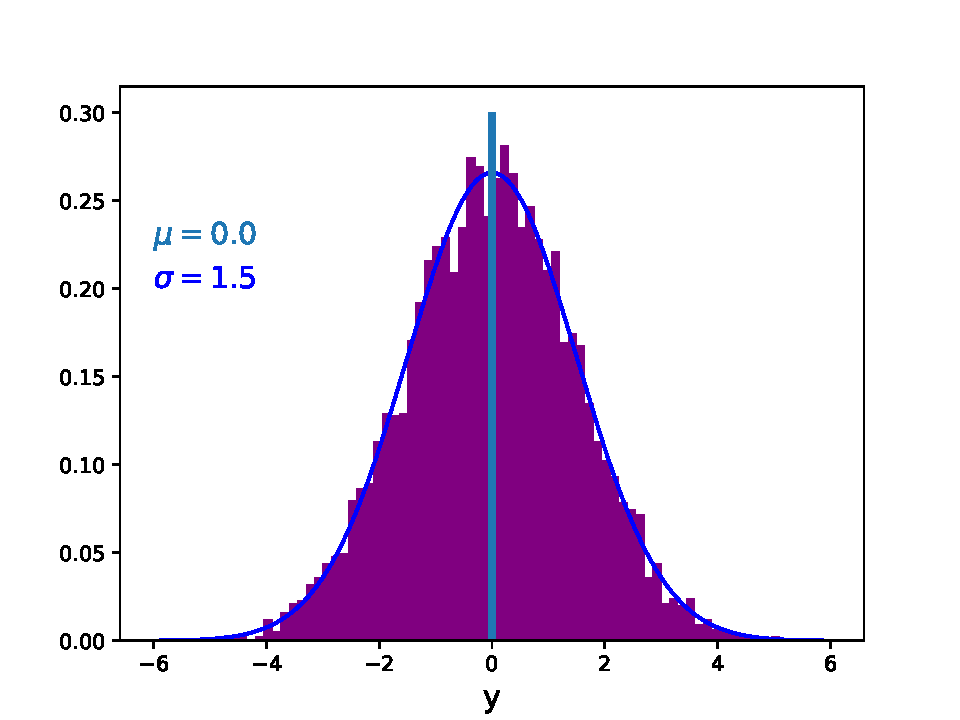
\includegraphics[scale=0.4]{gaussian_1d.pdf}
  \end{figure}
\end{frame}

\begin{frame}{\subsecname}
  

  Loi Gaussienne multidimensionnelle (\coloredemph{vecteur} Gaussien): Distribution \coloredemph{jointe} des composantes d'un vecteur $d$-dimensionnel dont les \coloredemph{marginales} sont Gaussiennes (unidimensionnelles).
  \begin{equation*}
    \vectorx{Y} := [ y_1, \dots, y_d ]^\top  \sim \mathcal{N}(\vectorx{\mu} , \matrixx{\Sigma}) =  \frac{1}{\sqrt{(2 \pi)^d \det |\matrixx{\Sigma}|}} e^{-\frac{1}{2}(\vectorx{y - \mu})^\top \matrixx{\Sigma}^{-1} (\vectorx{y - \mu})}
  \end{equation*}
% 
  \begin{enumerate}
    \item $\vectorx{\mu} \in \mathbb{R}^d$: \coloredemph{vecteur moyen} $\implies \mu_j$: moyenne de la Gaussienne $y_j$
    \item $\matrixx{\Sigma} \in \mathbb{R}^{d \times d}$ définie positive\footnote{i.e. $\vectorx{a}^\top \matrixx{\Sigma} \vectorx{a} > 0$ (donc symmétrique)}: \coloredemph{matrice de covariance}
  \end{enumerate}
% 
  \pause
  \begin{equation*}
    \matrixx{\Sigma}
    =
    \begin{pmatrix} 
      \Sigma^2_{1}  & \Sigma_{{1}{2}} &  \cdots & \Sigma_{{1}{d}} \\
      \Sigma_{{2}{1}} & \ddots          & \cdots  & \vdots \\
      \vdots          & \vdots          & \ddots  & \vdots \\
      \Sigma_{{d}{1}} & \cdots          & \cdots  &  \Sigma^2_{d} 
      \end{pmatrix}
    \implies
    \left\{
      \begin{array}{ll}
        \Sigma_j  : \text{écart-type} \text{ de } y_j\\
        \Sigma_{ij} : \text{covariance entre les } \\
        \text{marginales } y_i \text{ et } y_j
      \end{array}
    \right.
  \end{equation*}
  % $\mathcal{N}(\mu_1, \Sigma_1^2) \dots \mathcal{N}(\mu_d, \Sigma_d^2)$.
\end{frame}

% d=2, low correlation
\begin{frame}{\subsecname}
  % 
  Cas $d=2$:
  \begin{equation*}
    \vectorx{\mu}
    =
    \begin{pmatrix}
      \mu_1 \\
      \mu_2
    \end{pmatrix},
    \quad
    \matrixx{\Sigma}
    =
      \begin{pmatrix}
        \Sigma_{1} & \Sigma_{12} \\
        \Sigma_{21} & \Sigma_{2}
      \end{pmatrix}
    =
      \begin{pmatrix}
        1.5 & \color{red}\rho = -0.3 \\
        \color{red}\rho = -0.3 & 1.5
      \end{pmatrix}
  \end{equation*}
% 
  \begin{figure}
    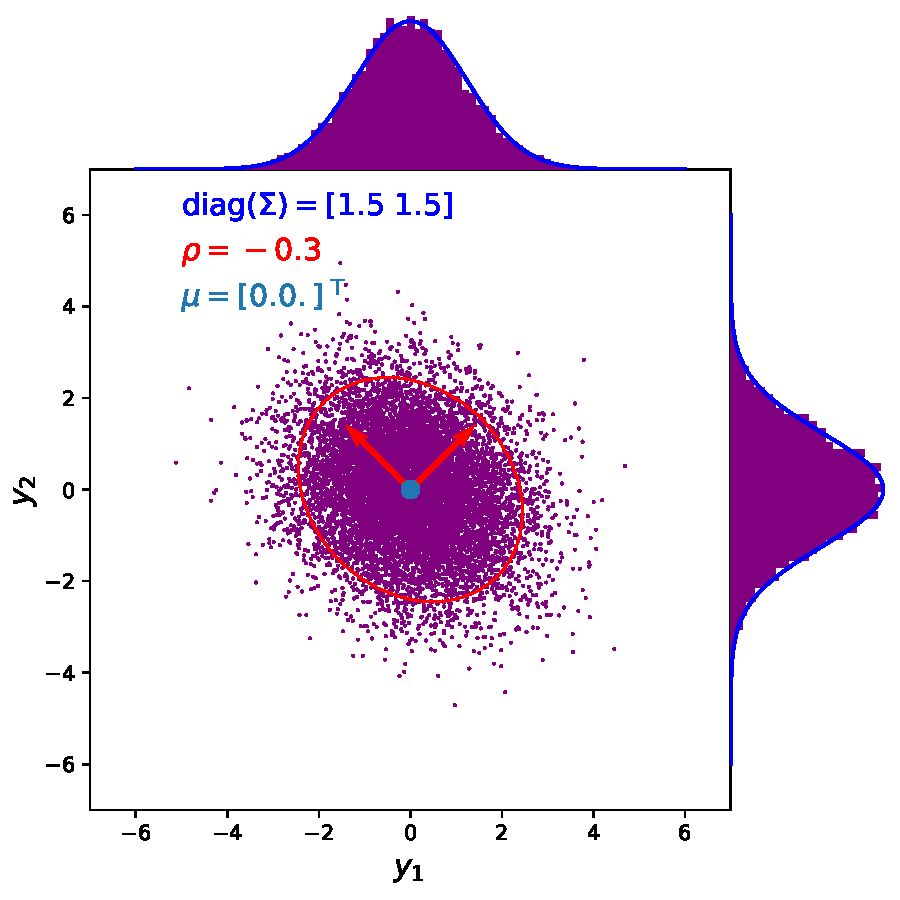
\includegraphics{gaussian_2d_rho_low.pdf}
  \end{figure}
\end{frame}

% d=2, high correlation
\begin{frame}{\subsecname}
  Cas $d=2$:
  %
  \begin{equation*}
    \vectorx{\mu}
    =
    \begin{pmatrix}
      \mu_1 \\
      \mu_2
    \end{pmatrix},
    \quad
    \matrixx{\Sigma}
    =
      \begin{pmatrix}
        \Sigma_{1} & \Sigma_{12} \\
        \Sigma_{21} & \Sigma_{2}
      \end{pmatrix}
    =
      \begin{pmatrix}
        1.5 & \color{red}\rho = 1.1 \\
        \color{red}\rho = 1.1 & 1.5
      \end{pmatrix}
  \end{equation*}
% 
  \begin{figure}
    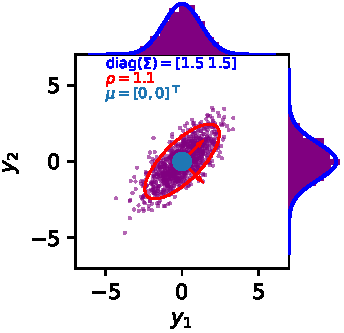
\includegraphics{gaussian_2d_rho_high.pdf}
  \end{figure}
\end{frame}

% d=2, zero correlation
\begin{frame}{\subsecname}
  Cas $d=2$:
  %
  \begin{equation*}
    \vectorx{\mu}
    =
    \begin{pmatrix}
      \mu_1 \\
      \mu_2
    \end{pmatrix},
    \quad
    \matrixx{\Sigma}
    =
      \begin{pmatrix}
        \Sigma_{1} & \Sigma_{12} \\
        \Sigma_{21} & \Sigma_{2}
      \end{pmatrix}
    =
      \begin{pmatrix}
        1.5 & \color{red}\rho = 0 \\
        \color{red}\rho = 0 & 1.5
      \end{pmatrix}
  \end{equation*}
% 
  \begin{figure}
    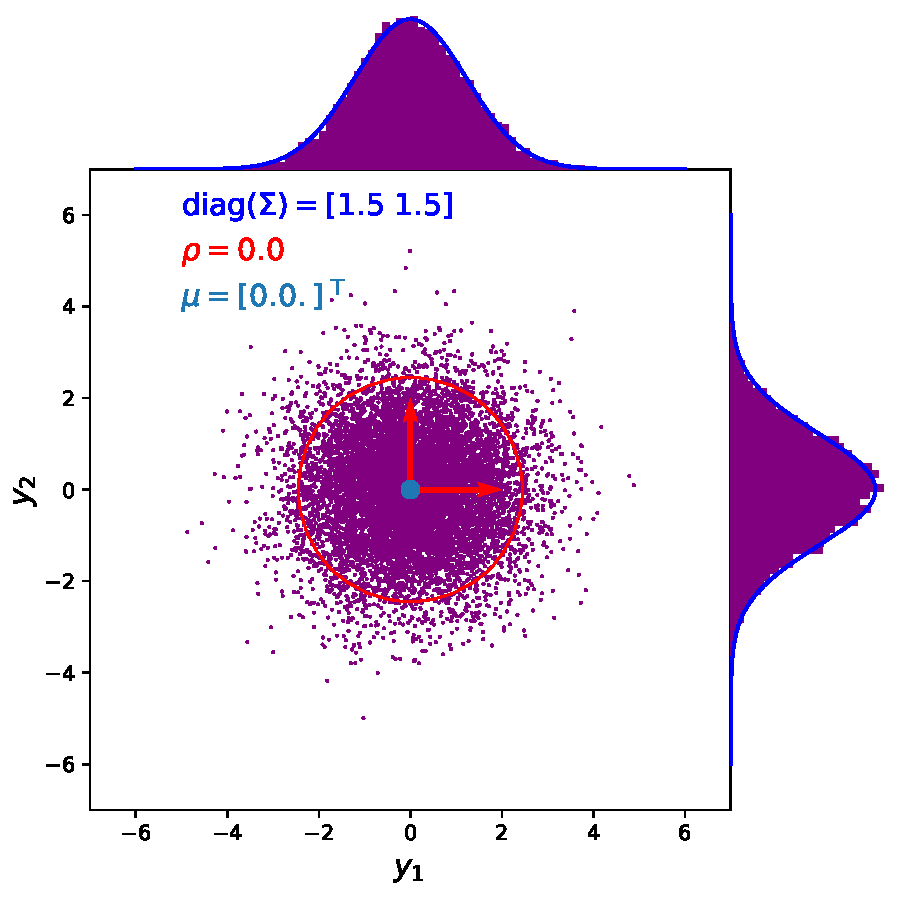
\includegraphics{gaussian_2d_rho_null.pdf}
  \end{figure}
\end{frame}

% d=5, high correlation: scatter and index plots
\begin{frame}{\subsecname}
  % 
  Cas $d=2$:
  %
  \begin{equation*}
    \vectorx{\mu}
    =
    \begin{pmatrix}
      0 \\
      0 \\
      \dots
    \end{pmatrix},
    \quad
    \matrixx{\Sigma}
    =
    \scalemath{0.5}{
      \begin{pmatrix}
        1.5 & 0.99 & \color{lightgray}0.98 & \color{lightgray}0.96 & \color{lightgray}0.94 \\
        0.99 & 1.5 & \color{lightgray}0.99 & \color{lightgray}0.98 & \color{lightgray}0.96 \\
        \color{lightgray}0.98 & \color{lightgray}0.99 & \color{lightgray}1.5 & \color{lightgray}0.99 & \color{lightgray}0.98 \\
        \color{lightgray}0.96 & \color{lightgray}0.98 & \color{lightgray}0.99 & \color{lightgray}1.5 & \color{lightgray}0.99 \\
        \color{lightgray}0.94 & \color{lightgray}0.96 & \color{lightgray}0.98 & \color{lightgray}0.99 & \color{lightgray}1.5
        \end{pmatrix}
    }
  \end{equation*}
  %
  \begin{figure}[ht]
    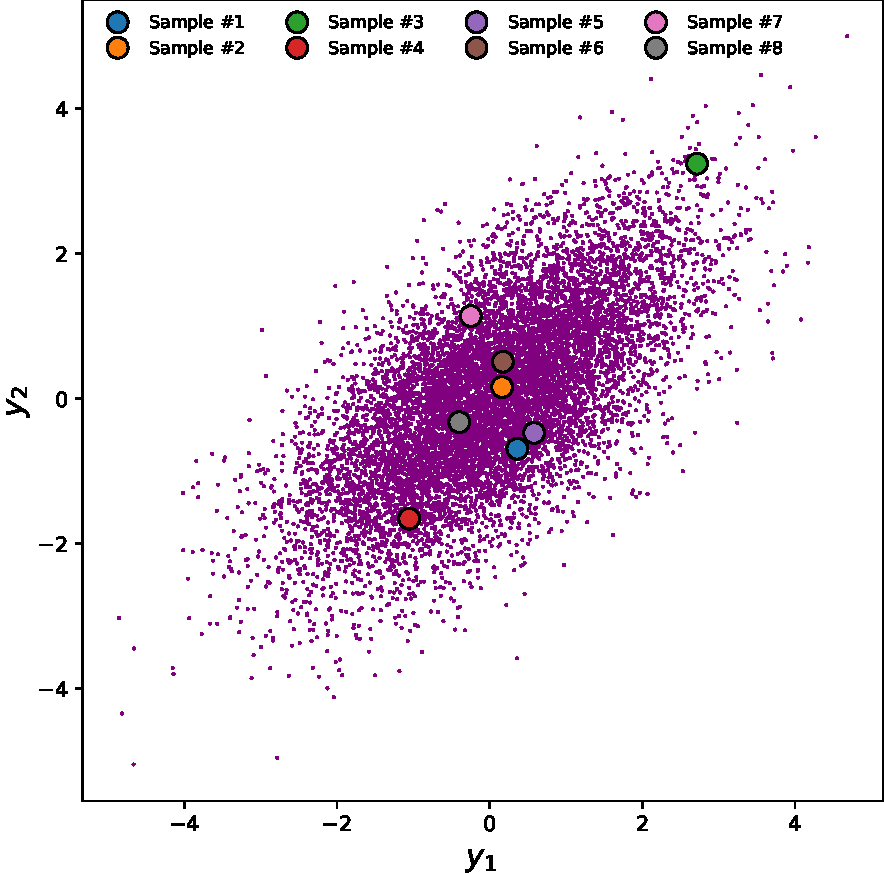
\includegraphics[scale=0.4]{gaussian_2d_2outof5.pdf}
    $\Longleftrightarrow$
    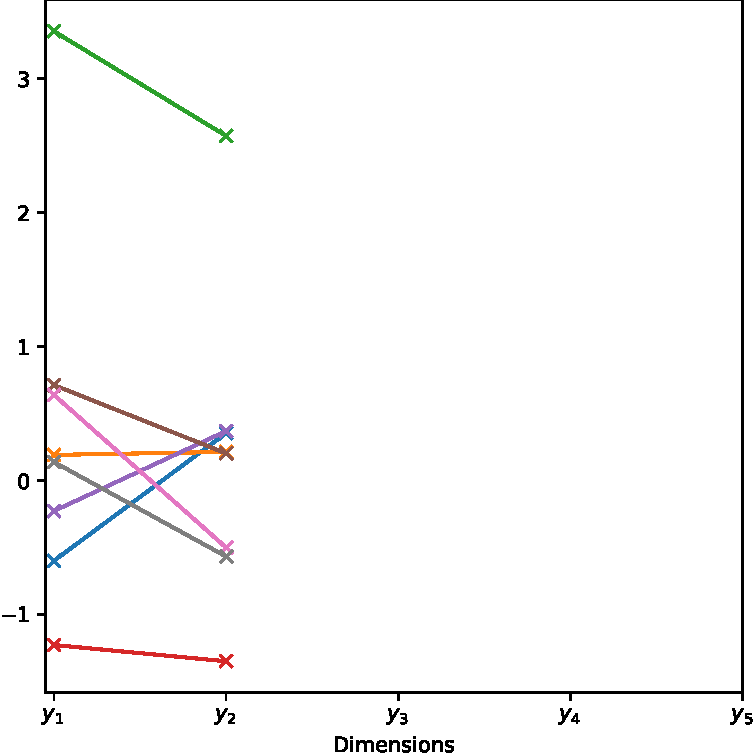
\includegraphics[scale=0.4]{gaussian_2d_valuevsindex.pdf}
    \caption{Dimensions $j=1, 2$. Gauche: \textcolor{violet}{$10^4$} $+8$ échantillons. 
    Droite: Réindéxation des $8$ \coloredemph{mêmes} échantillons.}
  \end{figure}
\end{frame}

% d=5, high correlation: scatter and index plots
\begin{frame}{\subsecname}
  Cas $d=5$:
  %
  \begin{equation*}
    \vectorx{\mu}
    =
    \begin{pmatrix}
      0 \\
      0 \\
      \dots
    \end{pmatrix},
    \quad
    \matrixx{\Sigma}
    =
    \scalemath{0.5}{
      \begin{pmatrix}
        1.5 & 0.99 & 0.98 & 0.96 & 0.94 \\
        0.99 & 1.5 & 0.99 & 0.98 & 0.96 \\
        0.98 & 0.99 & 1.5 & 0.99 & 0.98 \\
        0.96 & 0.98 & 0.99 & 1.5 & 0.99 \\
        0.94 & 0.96 & 0.98 & 0.99 & 1.5
        \end{pmatrix}
    }
  \end{equation*}
  %
  \begin{figure}[h]
    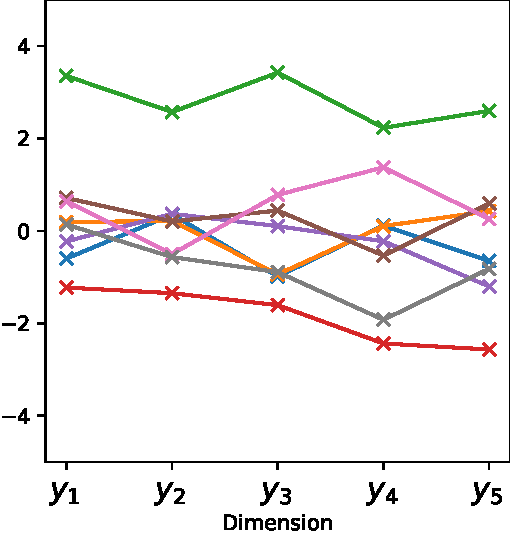
\includegraphics[scale=0.4]{gaussian_5d_valuevsindex.pdf}
    \caption{Réindéxation de $8$ échantillons, dimensions $j=1, \dots, 5$.
    Chaque "courbe" est un tirage de $\mathcal{N}(\vectorx{\mu} , \matrixx{\Sigma})$
    }
  \end{figure}
\end{frame}

% d=50, high correlation: scatter and index plots
\begin{frame}{\subsecname}
  Cas $d=50$:%
  \begin{equation*}
    \vectorx{\mu}
    =
    \begin{pmatrix}
      0 \\
      0 \\
      \dots
    \end{pmatrix},
    \quad
    \matrixx{\Sigma}
    =
    \scalemath{0.5}{
      \begin{pmatrix}
        1.5 & 0.998 & 0.993 & 0.986 & 0.975 & 0.962 & 0.946 & 0.927 & \cdots \\
        0.998 & 1.5 & 0.998 & 0.993 & 0.986 & 0.975 & 0.962 & 0.946 & \cdots \\
        0.993 & 0.998 & 1.5 & 0.998 & 0.993 & 0.986 & 0.975 & 0.962 & \cdots \\
        0.986 & 0.993 & 0.998 & 1.5 & 0.998 & 0.993 & 0.986 & 0.975 & \cdots \\
        0.975 & 0.986 & 0.993 & 0.998 & 1.5 & 0.998 & 0.993 & 0.986 & \cdots \\
        0.962 & 0.975 & 0.986 & 0.993 & 0.998 & 1.5 & 0.998 & 0.993 & \cdots \\
        0.946 & 0.962 & 0.975 & 0.986 & 0.993 & 0.998 & 1.5 & 0.998 & \cdots \\
        0.927 & 0.946 & 0.962 & 0.975 & 0.986 & 0.993 & 0.998 & 1.5   \\
        \hdots & \hdots & \hdots & \hdots & \hdots & \hdots & \hdots & \hdots & 1.5
      \end{pmatrix}
    }
  \end{equation*}%
  \begin{figure}[h]
    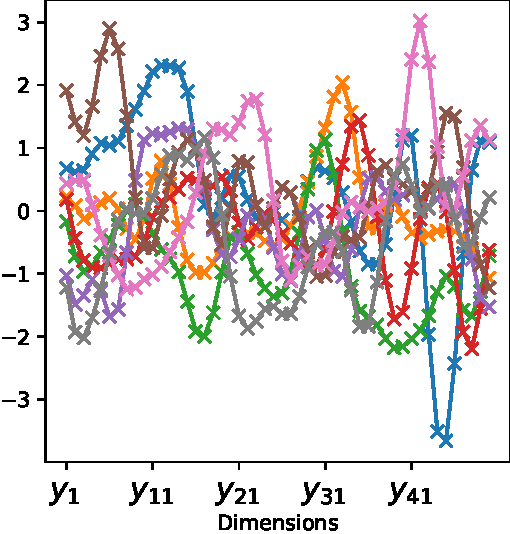
\includegraphics[scale=0.4]{gaussian_50d_valuevsindex.pdf}%
    \caption{Réindéxation de $8$ échantillons, dimensions $j=1, \dots, 50$}
  \end{figure}
\end{frame}
%

% GP definition
\begin{frame}{\subsecname}
  
  Cas $d=\infty$: chaque courbe est une \coloredemph{collection infinie} de valeurs, que l'on peut voir comme une fonction:%
  \begin{enumerate}
    \item $\vectorx{\mu}$: vecteur de taille infinie $\Leftrightarrow$ fonction moyenne $\mathbb{E}(y(x)) = m(\vectorx{x})$
    \item $\matrixx{\Sigma}$: matrice de taille infinie $\Leftrightarrow$  noyau de covariance ou "\coloredemph{kernel}"
    $\mathbb{C}( y(\vectorx{x}), y(\vectorx{x^\prime}) ) = k(\vectorx{x}, \vectorx{x^{\prime}})$
  \end{enumerate}
  % 
  \pause
  % 
  \begin{block}{Processus Gaussien $y(\vectorx{x}) \sim GP(m, k)$ \cite{Rasmussen2006}}
    Un processus Gaussien (GP) est une distribution de probabilités sur un espace de \coloredemph{fonctions},
    $y(\vectorx{x}): \mathcal{X} \to \mathcal{Y}$, telle que toute collection finie
    $[ y(x_i), \dots, y(x_j), \dots y(x_k) ], \forall i,j,k$ forme un vecteur Gaussien. 
    % Les deux fonctions $m$ et $k$ définissent les paramètres du $GP$.
  \end{block}
\end{frame}

\begin{frame}{\subsecname}
  \begin{itemize}
    \item $GP$ peut être vu comme une réindéxation d'un vecteur "infini"
    \pause
    \item Cas temporal: $y(t): \mathbb{R}^{+} \to \mathbb{R}$, \coloredemph{n'importe qu'elle discrétisation} de $y$ doit
    former un vecteur Gaussien, en prenant par ex $2$ entrées de $y$:
    \begin{equation*}
      y(\vectorx{x}) \sim GP(m, k) \implies
      y([t_i, t_j]) \sim \mathcal{N} (
        % mu
        \begin{pmatrix}
          \mu_i \\
          \mu_j 
        \end{pmatrix},
        % sigma
        \begin{pmatrix}
          \Sigma_{i}^2 & \Sigma_{ij} \\
          \Sigma_{ij} & \Sigma_{j}^2
        \end{pmatrix}
        )
    \end{equation*}
    \item Exemple visu: cf. exemples introductifs
  \end{itemize}
\end{frame}

\begin{frame}{\subsecname}
  \begin{itemize}
    \item Cas spatial: $y(\vectorx{x}): \mathbb{R}^2 \to \mathcal{Y} = \mathbb{R}$ (ex: température en 2D)
    \item Visu d'un échantillon:%
  \end{itemize}%
  \begin{figure}
    \centering
    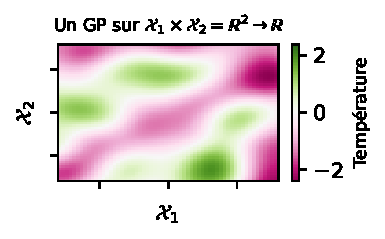
\includegraphics[scale=1]{1_gp_space_SquaredExponentialKernel.pdf}
  \end{figure}
\end{frame}

% informal details
\begin{frame}{\subsecname}
  \begin{itemize}
    \item On impose souvent une forme simple sur $\mathbb{E}(y(x)) = m(x)$ 
    comme: $\vectorx{\beta}^\top \vectorx{x}$, $\vectorx{0}$
    \pause
    \item $y: \mathcal{X} \to \mathcal{Y}$ est une \coloredemph{fonction}: il suffit de bien choisir $\mathcal{X}$ et $\mathcal{Y}$
    \begin{itemize}
      \item $\mathcal{X} = \mathbb{R}^{+}$ et $\mathcal{Y} = \mathbb{R}$ $\implies$
      $y$ = \coloredemph{série temporelle} \cite{Rasmussen2006}
      \pause
      \item $\mathcal{X} = [a, b] \times [c, d]$ (ou $\mathbb{R}^2$) et  $\mathcal{Y} = \mathbb{R}$ $\implies$
      $y$ = \coloredemph{champ spatial} (météo, hydro, etc)
      \pause
      \item $\mathcal{X} = [a, b] \times [c, d] \times \mathbb{R}^{+}$ et $\mathcal{Y} = \mathbb{R}$ $\implies$
      $y$ = \coloredemph{série temporelle d'images}
      \pause
      \item $\mathcal{X} = \mathbb{R}^{d}$ et $\mathcal{Y} = \{1 \dots K \}$ $\implies$
      $y$ = \coloredemph{classificateur} d'images/pixels (ex: segmentation) \cite{Hensman2015}
      \item $\mathcal{X}$ et $\mathcal{Y}$ peuvent être des espaces de graphes \cite{Borovitskiy2021}
      \item \dots etc, etc, etc.
    \end{itemize}
  \end{itemize}
  % 
\end{frame}

\subsection{Le kernel}
\begin{frame}{\subsecname}
  % 
  \begin{itemize}
    \item $k(\vectorx{x}, \vectorx{x^{\prime}}) = \mathbb{C}( y(\vectorx{x}), y(\vectorx{x^\prime}) )$
     représente la \coloredemph{similarité de $y$} entre deux entrées $\vectorx{x}$ et $\vectorx{x}^\prime$,
     donc doit générer une matrice de covariance valide%
     \footnote{
      $\sum_{i,j}^{n} a_i a_j k(\vectorx{x}_i, \vectorx{x}_j) \geq 0, \forall \vectorx{a} = [a_1, \dots, a_n]$
    }
    \pause
    \item $k$ défini \coloredemph{implicitement} les propriétés fonctionnelles de $y$%
    \footnote{
      C-à-d être un noyau reproduisant d'un espace de Hilbert:
      $y(x_0) = \sum_{i=1}^{\infty} y(x_i) k(x_i, x_0)$ 
    }
    \pause
    \item Kernel: fonction qui dépend aussi \coloredemph{d'hyperparamètres} $\vectorx{\theta}$
    \pause
    \item Et donc le nerf d'un $GP$ est essentiellement dans son kernel (noyau)
  \end{itemize}
\end{frame}

% Examples of kernel functions
\begin{frame}{\subsecname}
  \begin{itemize}
    \item Quelques exemples de $GP(0, k)$ défini sur $\mathcal{X} = \mathbb{R}^+$ et $\mathcal{Y} = \mathbb{R}$
    (série temporelle)
    %
    \item kernel de série temporelle $\leftrightarrow$ fonction d'\coloredemph{autocovariance}
    %
    \item Visualiser: bonne manière de comprendre un kernel
  \end{itemize}  
\end{frame}

% Exponential quadratic
\begin{frame}{\subsecname}
  \begin{itemize}
    \item<1-> Exponentiel quadratique (aka "Radial basis", "Gaussian", "Heat" kernel):
    $k (t, t^\prime) = e^{- \frac{(t - t^\prime)^2}{2 \ell^2} }$
    %
    \item<1-> $GP (0, k)$ génère des $y$ infiniment différentiables par rapport à $t$
    %
    \item<1-> $\ell$ contrôle le lissé (ici au sens oscillatoir) des générées
  \end{itemize}
  \begin{figure}
    \only<2>{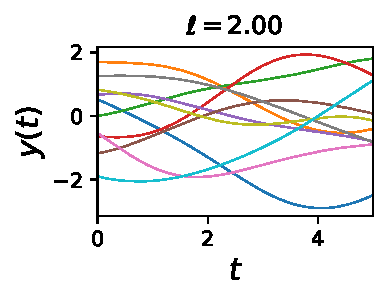
\includegraphics{10_gp_time_SquaredExponentialKernel_2.00.pdf}}%
    \only<3>{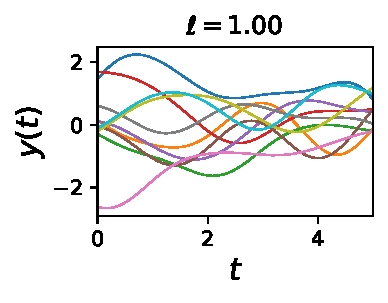
\includegraphics{10_gp_time_SquaredExponentialKernel_1.00.pdf}}%
    \only<4>{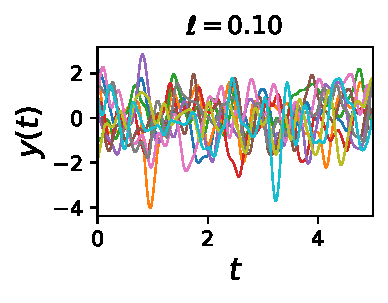
\includegraphics{10_gp_time_SquaredExponentialKernel_0.10.pdf}}%
  \end{figure}
\end{frame}

% Matern kernel
\begin{frame}{\subsecname}
  \begin{itemize}
    \item<1-> kernel de Matérn:
    $k (t, t^\prime) = ( 1 + \sqrt{\frac{3 |t - t^\prime|}{\ell} } ) e^{-\sqrt{\frac{3 |t - t^\prime|}{\ell} }}$
    %
    \item<1-> Génère des $y$ différentiables une seule fois par rapport à $t$
    %
    \item<1-> $\ell$: même interprétation que le kernel exponentiel quadratique
  \end{itemize}
  \begin{figure}
    \only<2>{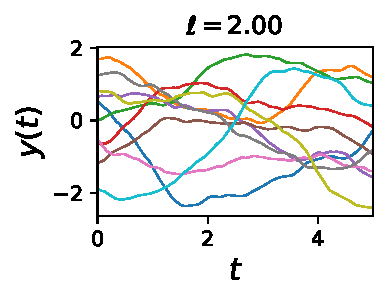
\includegraphics{10_gp_time_MaternKernel_2.00.pdf}}%
    \only<3>{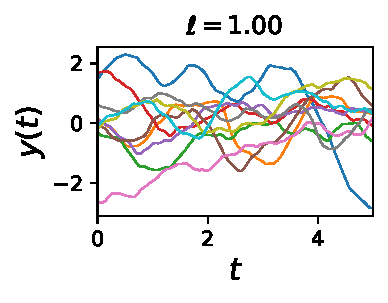
\includegraphics{10_gp_time_MaternKernel_1.00.pdf}}%
    \only<4>{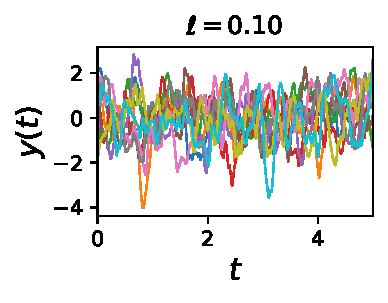
\includegraphics{10_gp_time_MaternKernel_0.10.pdf}}%
  \end{figure}
\end{frame}

% Locally periodic
\begin{frame}{\subsecname}  
  % 
  \begin{itemize}
    \item<1-> kernel locallement-périodique:
    $k (t, t^\prime) = e^{- \frac{2 \sin^2(\pi (t - t^\prime) / T_0)}{\ell^2}}$
    %
    \item<1-> Génère des $y$ périodiques ET lisses
  \end{itemize}
  \begin{figure}
    \only<2>{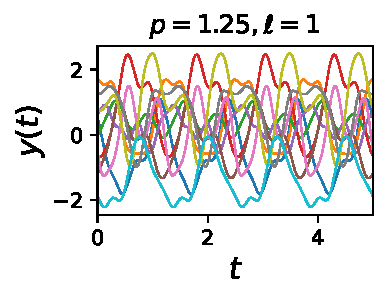
\includegraphics{10_gp_time_PeriodicKernel_1.25.pdf}}%
    \only<3>{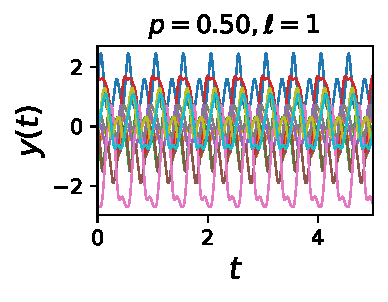
\includegraphics{10_gp_time_PeriodicKernel_0.50.pdf}}%
  \end{figure}
\end{frame}

% White noise kernel
\begin{frame}{\subsecname}
  \begin{itemize}
    \item<1-> kernel de bruit blanc: 
    \begin{equation*}
        k(t, t^\prime) = 
        \left\{
          \begin{array}{ll}
            \sigma^2  \text{ si } t = t^\prime \\
            0 \text{ sinon }
          \end{array}
        \right.
    \end{equation*}
    %
    \item<1-> Aucune corrélation. $\sigma$ contrôle l'amplitude (variance) du bruit
  \end{itemize}
  \begin{figure}
    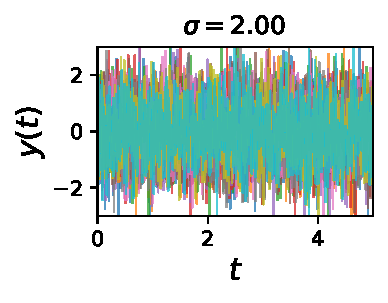
\includegraphics{10_gp_time_WhiteKernel_2.00.pdf}%
  \end{figure}
\end{frame}

\begin{frame}{\subsecname}
  \begin{itemize}
    \item Aussi, des kernels dans le domaine fréquentiel (Fourier)\cite{Parra2017}%
    \footnote{ex: $\sum_{q=0}^Q \sigma_q^2 e^{-2 \pi^2 \Sigma_q (t-t^\prime)^2} \cos(2\pi \mu_q (t-t^\prime))$}
  %  
  \pause
    \item Famille des \coloredemph{kernels stationnaires}, 
    $k(t, t^\prime)$ ne dépend que de $t - t^\prime \leftrightarrow$ "plus les inputs sont éloignées, moins les sorties associées sont corrélées"
  \end{itemize}
  %
  \begin{figure}
    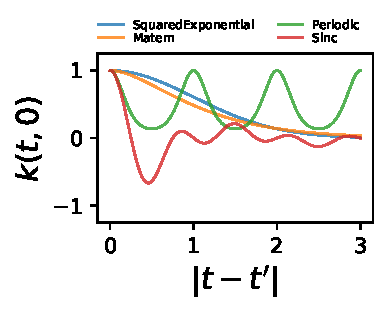
\includegraphics[scale=0.80]{autocov_gp_1D.pdf}
  \end{figure}
\end{frame}

\begin{frame}{\subsecname}
  \begin{itemize}
    \item Fléxibilité des kernels: $k_1 + k_2$, $k_1 \times k_2$, $g(t) \times k$ ($g$ est déterministe)
  \pause
    \begin{itemize}
      \item $k_1 + k_2$: "Ou" logique
      \item $k_1 \times k_2$: "Et" logique
    \end{itemize}
    %
    \item Depuis quelques années: construction de kernels par des deep-nets \cite{Wilson2016}, pratique mais peu interprétable% 
  \pause
    \item Plus récemment: construction de kernel à  partir d'équations différentielles
  \end{itemize}
\end{frame}

%========== Fitting a GP ==================%
\section{Prédire avec un $GP$}
% Gaussian Bayesian rule
\subsection{Règle de Bayes}
\begin{frame}{\subsecname}  
  \begin{itemize}
    \item<1-> Règle de Bayes: %
    $p(y_2| y_1)
    = \frac{p(y_1, y_2)}{p(y_1)}
    = \frac{p(y_1 | y_2) p(y_2)}{p(y_1)}
    $%
    \item<2-> $  \vectorx{y} = [y_1, y_2]^\top \sim \mathcal{N} (
      \begin{pmatrix}
        \mu_1 \\
        \mu_2
      \end{pmatrix},
        \begin{pmatrix}
          \Sigma_{1} & \rho \\
          \rho & \Sigma_{2}
        \end{pmatrix}
    )$%
    \item<3-6> $
    p(y_2 | y_1 = u) = \mathcal{N} (
      \mu_2 \tored{+ \rho \Sigma_1^{-1} (u - \mu_1)},
      \Sigma_2 \tored{- \rho^2 \Sigma_1^{-1}}%
    )$%
  \end{itemize}%
  \begin{figure}
    \centering
    \only<4>{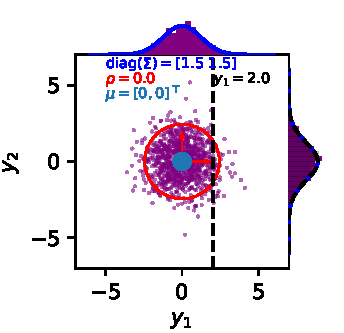
\includegraphics{gaussian_2d_rho_null_with_conditional.pdf}}%
    \only<5>{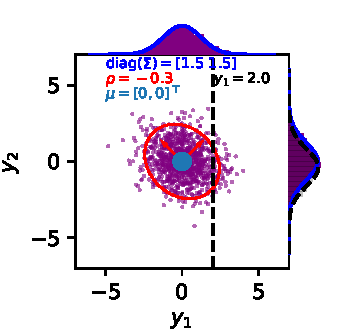
\includegraphics{gaussian_2d_rho_low_with_conditional.pdf}}%
    \only<6>{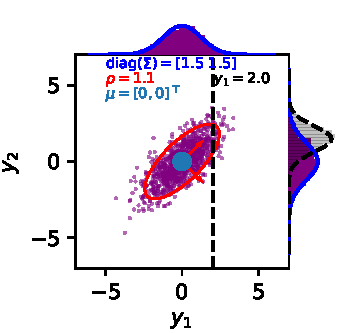
\includegraphics{gaussian_2d_rho_high_with_conditional.pdf}}%
  \end{figure}
  \only<7>{
    $
    p(y_2 | y_1 = u) = \mathcal{N} (
      \mu_2 \tored{+ \rho \Sigma_1^{-1} (u - \mu_1)},
      \underbrace{\Sigma_2 \tored{- \rho^2 \Sigma_1^{-1}}}_{\geq 0}%
    )$%
    \\
    Conditionner $y_2 | y_1$ $\leftrightarrow$ réduire l'incertitude (variance) de $y_2$
    \\
    \pause
    Conditionnement entre variables Gaussiennes: reste Gaussien (conjugué)
    }%
\end{frame}

% Posterior of a GP
\subsection{prédiction $=$ data $\times$ hypothèse}
\begin{frame}{\subsecname}
  
  \begin{itemize}
  \item<1-> Data \tored{entraînement}: $\{y_i, x_i\}_{1 \leq i \leq n} = [\tored{y}, \tored{\vectorx{x}}]$, test: $y_0, \toblue{x_0}$%
  \item<2-> Modèle de \toblue{prédiction} (régression): $y_0 = f_{\theta}(x_0)$ %(pour le moment sans bruit)%
  \item<3-> \topurple{Hypothèses}: $\topurple{f_\theta} \sim GP(0, k_\theta)$ et $y_i = f_\theta (x_i)$:%
  \begin{equation*}
    \underbrace{[\tored{y}, f_\theta( \toblue{x_0} )]^\top}_{(n + 1) \times 1} \sim \mathcal{N}(
      % mean
      \vectorx{0},
      % kernel
      % k_\theta(\tored{\vectorx{x}}, \tored{\vectorx{x}})
    \begin{pmatrix}
      \matrixx{K}_{\tored{y}}   & \vectorx{k}_{\toblue{0}} \\
      \vectorx{k}_{\toblue{0}}^\top      & k_\theta( \toblue{x_0} , \toblue{x_0} )
    \end{pmatrix}
    )
  \end{equation*}
  %
  \only<4>{
    \matrixx{K}_{\tored{y}} =
    \scalemath{0.80}{
    \begin{pmatrix}
      k_\theta(\tored{x_1}, \tored{x_1}) & \dots & k_\theta(\tored{x_1}, \tored{x_n}) \\
      \vdots             & \ddots& \vdots          \\
      k_\theta(\tored{x_n}, \tored{x_1}) & \dots & k_\theta(\tored{x_n},\tored{x_n})
    \end{pmatrix}}
  }
  \only<5>{
    $\vectorx{k}_{\toblue{0}} = [k_\theta(\toblue{x_0}, \tored{x_1}), \dots, k_\theta(\toblue{x_0}, \tored{x_n})]^\top$
  }
  %
  \item<6-> But: aprendre $f_\theta$ $\rightarrow$ prédire $f_\theta (x_0) = y_0$
  %
  \item<6-> Intuitivement: générer des \coloredemph{prédictions} avec $f_\theta \sim GP (0, k_\theta)$
  ET garder ce qui fit à $[\tored{y}, \tored{\vectorx{x}}]$ et à \coloredemph{$x_0$}:
  %
  \only<7>{
    $\underbrace{p(hypothèse | data)}_{\toblue{posterior}}
    & = 
    \frac{
      \overbrace{p(data | hypothèse)}^{\tored{likelihood}}
      \overbrace{p(hypothèse)}^{\topurple{prior}}
    }{
      \underbrace{p(data)}_{evidence}
    }$}
  %
  \item <8-> Revient à générer selon:%
    \begin{equation*}
      \only<8->{
        \overbrace{p( f_{\theta}( \tored{\vectorx{x}} ), f_{\theta}( \toblue{x_0} ) | \tored{y}, \tored{\vectorx{x}}, x_0)}^{\toblue{posterior}}
      }
      \only<9->{
        =
        \frac{
          \overbrace{p(\tored{y} | f_{\theta} (\tored{\vectorx{x}}) )}^{\tored{likelihood}}
          \overbrace{p( f_{\theta}( \tored{\vectorx{x}} ), f_{\theta}( \toblue{x_0} ) )}^{\topurple{prior}}
        }{
          p(\tored{y} | \tored{\vectorx{x}})
        } 
        = GP(
          m_{*},
          k_{*, \theta}
        )
      }
    \end{equation*}
\end{itemize}
\end{frame}

\begin{frame}{\subsecname}
  \toblue{Prédiction} (aka inférence):
  \begin{itemize}
    \item<1-> $m_{*}, k_{*, \theta}$ ?
    \item<1-> $p(f_\theta | y, \vectorx{x}) = GP(m_{*}, k_{*, \theta})$
     % posterior mean
    \item<2-> $m_*(\toblue{x_0}) = 0 +$
    \only<3-> $\vectorx{k}_{\toblue{0}}^\top \tored{\matrixx{K}_{y}}^{-1} \tored{y}$
     % posterior covariance
    \item<4-> $k_{*, \topurple{\theta}} (\toblue{x_0}, x_0^\prime) = k_\topurple{\theta} (\toblue{x_0}, x_0^\prime) -$
    \only<5->{$\vectorx{k}_{\toblue{0}}^\top \tored{\matrixx{K}_{y}}^{-1} \vectorx{k}_{\toblue{0}}$}
    %
    \item<6-> La distribution de probabilités de la prédiction $y_0$ (connaissant les data d'entraînement) est caractérisée !
    %
    \item<6-> Pour n'importe quel $x_0$: accès à la prédiction moyenne, incertitude (intervalle de confiance), quantiles, etc., de $y_0$
    %
    \item<7-> Modèle de prédiction = \{ data d'\tored{entraînement}, hyperparamètres \}
    %
    \item<8-> La prédiction dépend aussi de $\topurple{\theta}$ (hyperparamètre) !
  \end{itemize}
\end{frame}

\begin{frame}{\subsecname}
  \tored{Entraînement}:
  \begin{itemize}
    \item<1-> Meilleur $\theta$ ?%
    \item<2-> Maximum de $\tored{likelihood}(\theta) := p(y | f_{\theta}(\vectorx{x}))$ ?
    \item<3-> NON !! Restreint l'\topurple{hypothèse} uniquement à $[\tored{y}, \tored{\vectorx{x}}]$ (overfitting)
    \item<4-> Mieux: \topurple{hypothèse} sur les data + voisinage
    \item<4-> Maximum de $\tored{likelihood} \tored{marginale}$: %
    \begin{align*}
      \only<6->{p( \tored{y} | \tored{\vectorx{x}}, \theta)}%
      \only<5>{
      &= p(\tored{y} | \topurple{f_{\theta}} ( \tored{\vectorx{x}} ) ) p( \topurple{f_{\theta}} ( \tored{\vectorx{x}} ) ) \\ }
      \only<6->{
        &=  \int_{\mathbb{R}^n} p(\tored{y} | \tored{\vectorx{x}}, \topurple{f_{\theta}} ( \tored{\vectorx{x}} ) ) p( \topurple{f_{\theta}} ( \tored{\vectorx{x}} ) ) \mathrm{d} \topurple{f_{\theta}}  \\ }
      \only<7->{
      &= \int \mathcal{N} ( \topurple{f_{\theta}} ( \tored{\vectorx{x}} ),  I_d ) \mathcal{N} (\vectorx{0}, \tored{\matrixx{k}_{y}} )\mathrm{d}f_{\theta}}
    \end{align*}
    % $ = \prod_{i} p( y_i | \vectorx{x}_i, f_\theta(\vectorx{x}_i) )$
    \item<5-> $\leftrightarrow$ $\theta$ telle que les données d'entraînement $\tored{y}$
    soient le plus probables au regard de toutes les des \topurple{hypothèses} possibles et des inputs $\tored{\vectorx{x}}$
  \end{itemize}
\end{frame}

\begin{frame}{\subsecname}
  \begin{itemize}
    \item<1->
     \begin{align*}
      \log \tored{likelihood marg}(\theta)
       &= \log p( \tored{y} | \tored{\vectorx{x}}, \theta) ( = \log \prod_{i} p( \tored{y_i} | \tored{x_i}, \theta) ) \\
       &= \log \mathcal{N} (\vectorx{0}, \tored{\matrixx{K}_y} + I_d) \\
       &= - \underbrace{ \tored{y}^\top \tored{\matrixx{K}_{y}}^{-1} \tored{y} }_{fidélité}
       - \underbrace{ \frac{1}{2} \log | \tored{\matrixx{K}_{y}} |}_{pénalité}
       - \frac{n}{2} \log 2 \pi
     \end{align*}    
   \item<2-> Rappel: %
   $\tored{\matrixx{K}_{y}}$ matrice $n \times n$ des $k_\theta(x_i, x_j) = \mathbb{C}(f_\theta(x_i), f_\theta(x_j)) \overset{ex}{=} e^{- \frac{(x_i - x_j)^2}{2 \ell^2} }$
   \item<3-> Apprentissage de $\theta$ par descente de gradient de $- \log \tored{likelihood marg}$ (large sous-domaine de la communauté GP)
  \end{itemize}
\end{frame}

\begin{frame}\frametitle{\secname}
  Méthodo générale:
  \begin{enumerate}
    \item Collecter des données: $\{y_i, x_i\}_{1 \leq i \leq n} = [\tored{y}, \tored{\vectorx{x}}]$
    \pause
    \item Formuler des \topurple{hypothèses}: choisir/combiner un/des kernels $\topurple{k}_{\theta}$
    \pause
    \item \tored{Entraîner} le modèle: estimer les hyperparamètres $\theta$
    \pause
    \item \toblue{Prédire} ("\emph{inférence}"): évaluer $m_*$ et $k_{*, \theta}$, générer des données, etc.
    \pause
    \item Critique/évaluation du modèle
  \end{enumerate}
\end{frame}

% Example
\subsection{Exemples}
\begin{frame}{\subsecname}
  \begin{itemize}
    \item\tored{train} = $\{y_i, x_i\}_{i \leq n}$ où $y_i = g(x_i) = - \cos(3 \pi x_i) + \frac{1}{4} \sin(8 \pi x_i)$
    %
    \item $g$ inconnue
      \begin{figure}
        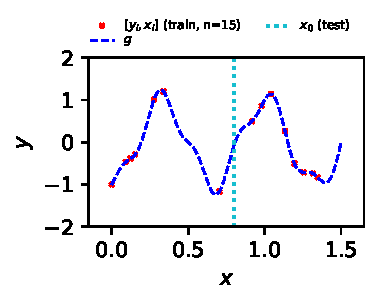
\includegraphics{gp_1D_example_noisefree_data.pdf}
      \end{figure}
    %[y_0]
    \item $f_\theta(x_0 = 0.8) = \tilde{y}_0$ ? (\coloredemph{interpolation})
  \end{itemize}
\end{frame}

\begin{frame}{\subsecname}
  \begin{itemize}
    \item<1-> \topurple{Hypothèses}: $y_i = f(x_i)$ et $f$ est lisse $\rightarrow$ kernel exponentiel quadratique
    %
    \item $k_\theta (x, x^\prime) = \sigma_k^2 e^{- \frac{(x - x^\prime)^2}{2 \ell^2} }, \theta = [\sigma_k, \ell]$
    %
    \item<2-> $[\sigma_k, \ell]$ inconnus (ici fixés arbitrairement)
      \begin{figure}
        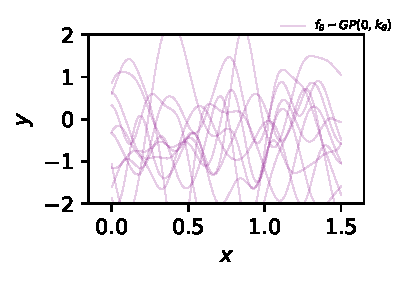
\includegraphics{gp_1D_example_noisefree_data_prior.pdf}
      \end{figure}    
  \end{itemize}
\end{frame}

\begin{frame}{\subsecname}
  \tored{Entraînement}
  \begin{itemize}
    \item<1-> $\theta$ ? minimisation de $-\log$ likelihood marginale: $\sigma_k \approx 0.92, \ell \approx 0.11$
    %
    \item<2-> $m_{*}, k_{*, \theta}$ et $\theta$ appris
    % 
    \item<3-> \toblue{Inférence}: générer selon la distribution posterior $GP( m_{*}, k_{*, \theta} )$
      \begin{figure}
        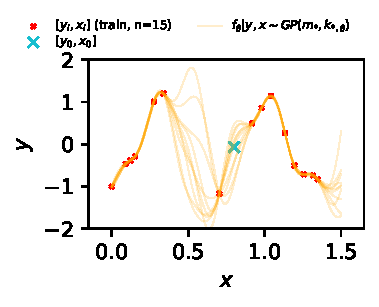
\includegraphics{gp_1D_example_noisefree_pred.pdf}
      \end{figure}
  \end{itemize}
\end{frame}

\begin{frame}{\subsecname}
  \toblue{{Inférence}}
  \begin{itemize}
    \item $\tilde{y}_0$: moyenne de $p(f_\theta | y, \vectorx{x}, x_0) = GP(m_{*}, k_{*, \theta})$ en $x_0 =0.8$
    %
    \item $m_{*}(x_0) \pm \frac{1}{2} \sqrt{k_{*, \theta}(x_0, x_0)}$: $ = -0.22 \pm 0.16$ ($95\%$)
  \end{itemize}
\end{frame}

\begin{frame}{\subsecname}
  \begin{itemize}
    \item Quid d'autres valeurs de $x_0$ ?
      \begin{figure}
        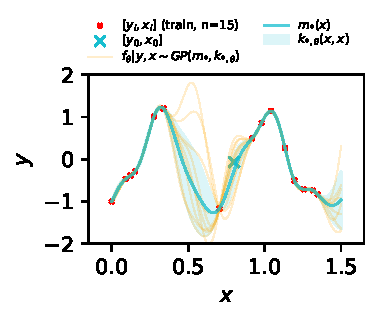
\includegraphics{gp_1D_example_noisefree_pred_meanvar.pdf}
      \end{figure}
    %
    \item Incertitude sur "toute" la fonction
  \end{itemize}
\end{frame}

\begin{frame}{\subsecname}
  \begin{itemize}
    \item \topurple{Hypothèses} précédentes: "pas de bruit" (hypothèse forte), "lisse" (hypothèse large)
    %
    \pause
    \item \topurple{Hypothèses} plus réalistes ?
    %
    \pause
    \item Bruit de mesure $y_i = f_{\theta}(x_i) + \epsilon$, lisse, quasi-périodique: $k_{\theta} = k_{\epsilon} + \sigma_{exp2} k_{exp2} \times \sigma_{per} k_{per}$
      \begin{itemize}
        \item $k_{\epsilon}$: bruit
        \item $k_{exp2} \times k_{per}$: Lisse ET quasi-périodique
        \item $\theta = [\sigma_{\epsilon}, \sigma_{exp2}, \ell, \sigma_{per}, T_0, \ell_{per}]$
      \end{itemize}
  \end{itemize}
\end{frame}

\begin{frame}{\subsecname}
  \begin{itemize}
    \item Même données + bruit blanc ($\sigma = 0.3$)
    \item $f_\theta(x_0 = 0.8) = \tilde{y}_0$ (\coloredemph{smoothing}) ?
  \end{itemize}
  \begin{figure}
    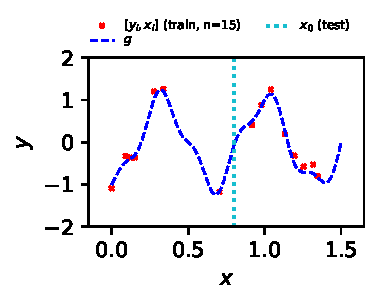
\includegraphics{gp_1D_example_noisy_data.pdf}
  \end{figure}
\end{frame}

\begin{frame}{\subsecname}
  \begin{itemize}
    \item<1-> $\theta$ ? minimisation de $-\log$ likelihood:
    $\sigma_{\epsilon} \approx 0.24$, $\sigma_{exp2} \approx 1$, $\ell \approx 1$, $\sigma_{per} \approx 1$, $T_0 = 0.7$, $\ell_{per} \approx = 1$
    %
    \item<2-> $m_{*}, k_{*, \theta}$ et $\theta$ appris
    % 
    \item<3-> Génération selon la distribution posterior $GP( m_{*}, k_{*, \theta} )$
      \begin{figure}
        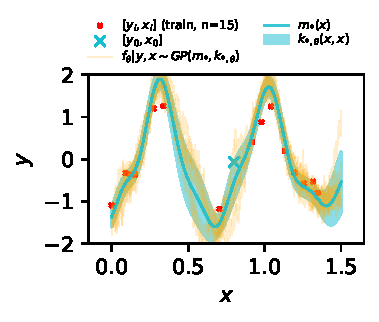
\includegraphics{gp_1D_example_noisy_pred_meanvar.pdf}
      \end{figure}
  \end{itemize}
\end{frame}
\begin{frame}{\subsecname}
  \begin{itemize}
    \item<1-> Pour $x > 1.5$ ? (\coloredemph{forecast})
    \item<2-> Comparaison des deux hypothèses
      \begin{figure}
        \centering
        \subfigure{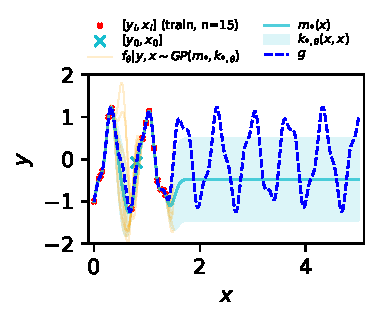
\includegraphics[scale=0.8]{gp_1D_example_noisefree_pred_meanvar_forecast.pdf}}
        \subfigure{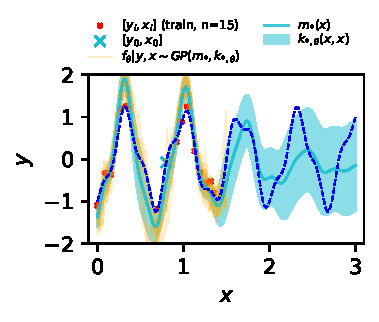
\includegraphics[scale=0.8]{gp_1D_example_noisy_pred_meanvar_forecast.pdf}}
        \caption{(a): sans bruit, lisse (b): bruit, lisse et périodique}
      \end{figure}
  \end{itemize}
\end{frame}

% %========== Motivations ==================%
% \section{Motivations}
% \subsection{Tractabilité mathématique}

% % Mathematical properties
% \begin{frame}{\subsecname}
  
% $y_1 \sim GP$, $y_2 \sim GP$
% \begin{itemize}
%   \pause
%   \item Somme: $y_1 + y_2 \sim GP$
%   %
%   \pause
%   \item Opérateur linéaire $\mathcal{L}$ (gradient, $\int$, eq-diff linéaire, etc.):
%   $\mathcal{L}y_1 \sim GP$
%   % 
%   \item Bayésien $\implies$ probabiliste: accès à l'incertitude de prédiction
%   \pause
%   \item Conditionnement Bayésien: $y_1 | y_2 \sim GP$ (\coloredemph{important}, détails plus tard)
%   % 
%   \pause
%   \item Connaissant uniquement moyenne et covariance de $\vectorx{u}$ et $\vectorx{v}$,
%   on montre que la meilleure prédiction (en moyenne) est Gaussienne (maximum d'entropie).
% \end{itemize}
% \end{frame}

% % Non-parametric
% \subsection{Non-paramétrique}
% \begin{frame}{\subsecname}
  
%     \begin{itemize}
%     \item Modèle \coloredemph{paramétrique}: modèle = des paramètres
%     \item Les données d'entraînement \coloredemph{conditionnent} les paramètres qui conditionnent eux-mêmes l'inférence (lien indirect)
%     \pause
%     \item Ex: régression linéaire, réseau de neurones (poids), K-means, RF
%     \pause
%     \item Modèle \coloredemph{non-paramétrique}: modèle = des données
%     \item Les données d'entraînement \coloredemph{conditionnent} l'inférence (lien direct)
%     \pause
%     \item Ex: SVM, k-NN, \coloredemph{GP} ($\coloredemph{\matrixx{K}_{fn}^{-1}}$)
%     \pause
%     %
%     \item Avantages du non-paramétrique:
%       \begin{enumerate}
%         \item apprentissage "direct" de la distribution des observations
%         \item théorie: $n \to \infty$: le modèle se trompe de moins en moins (pas toujours le cas du paramétrique)
%         \item inférence Gaussienne optimale\footnote{à partir de moyenne et covariance uniquement.}
%       \end{enumerate}
%     \pause
%     %
%     Inconvénivents du non-paramétrique:
%       \begin{enumerate}
%         \item risque d'overfit plus important
%         \item variance de prédiction sensible aux hyperparamètres du kernel
%         \item inférence plus coûteuse en général
%       \end{enumerate}
%   \end{itemize}
% \end{frame}

%========== Application ==================%
\subsection{Application: prédiction de température maritime}

\begin{frame}{\subsecname}
  \begin{itemize}
    \item<1-> Séries temporelles de température sur la côté sud anglaise\footnote{\href{https://www.bramblemet.co.uk/(S(oqanew55msnsth55kvmmlxu2))/default.aspx}{Accessible ici}}:
    4 stations sur 7 jours, $\Delta t \approx 5$min
    \only<1>{
        \begin{figure}
        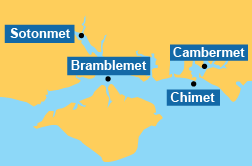
\includegraphics[scale=0.8]{ukcoast_map.png}
      \end{figure}
    }
    \item<2-> But: estimation du bruit, forecasting et complétion de valeurs manquantes
    \begin{figure}
      \centering
      \subfigure{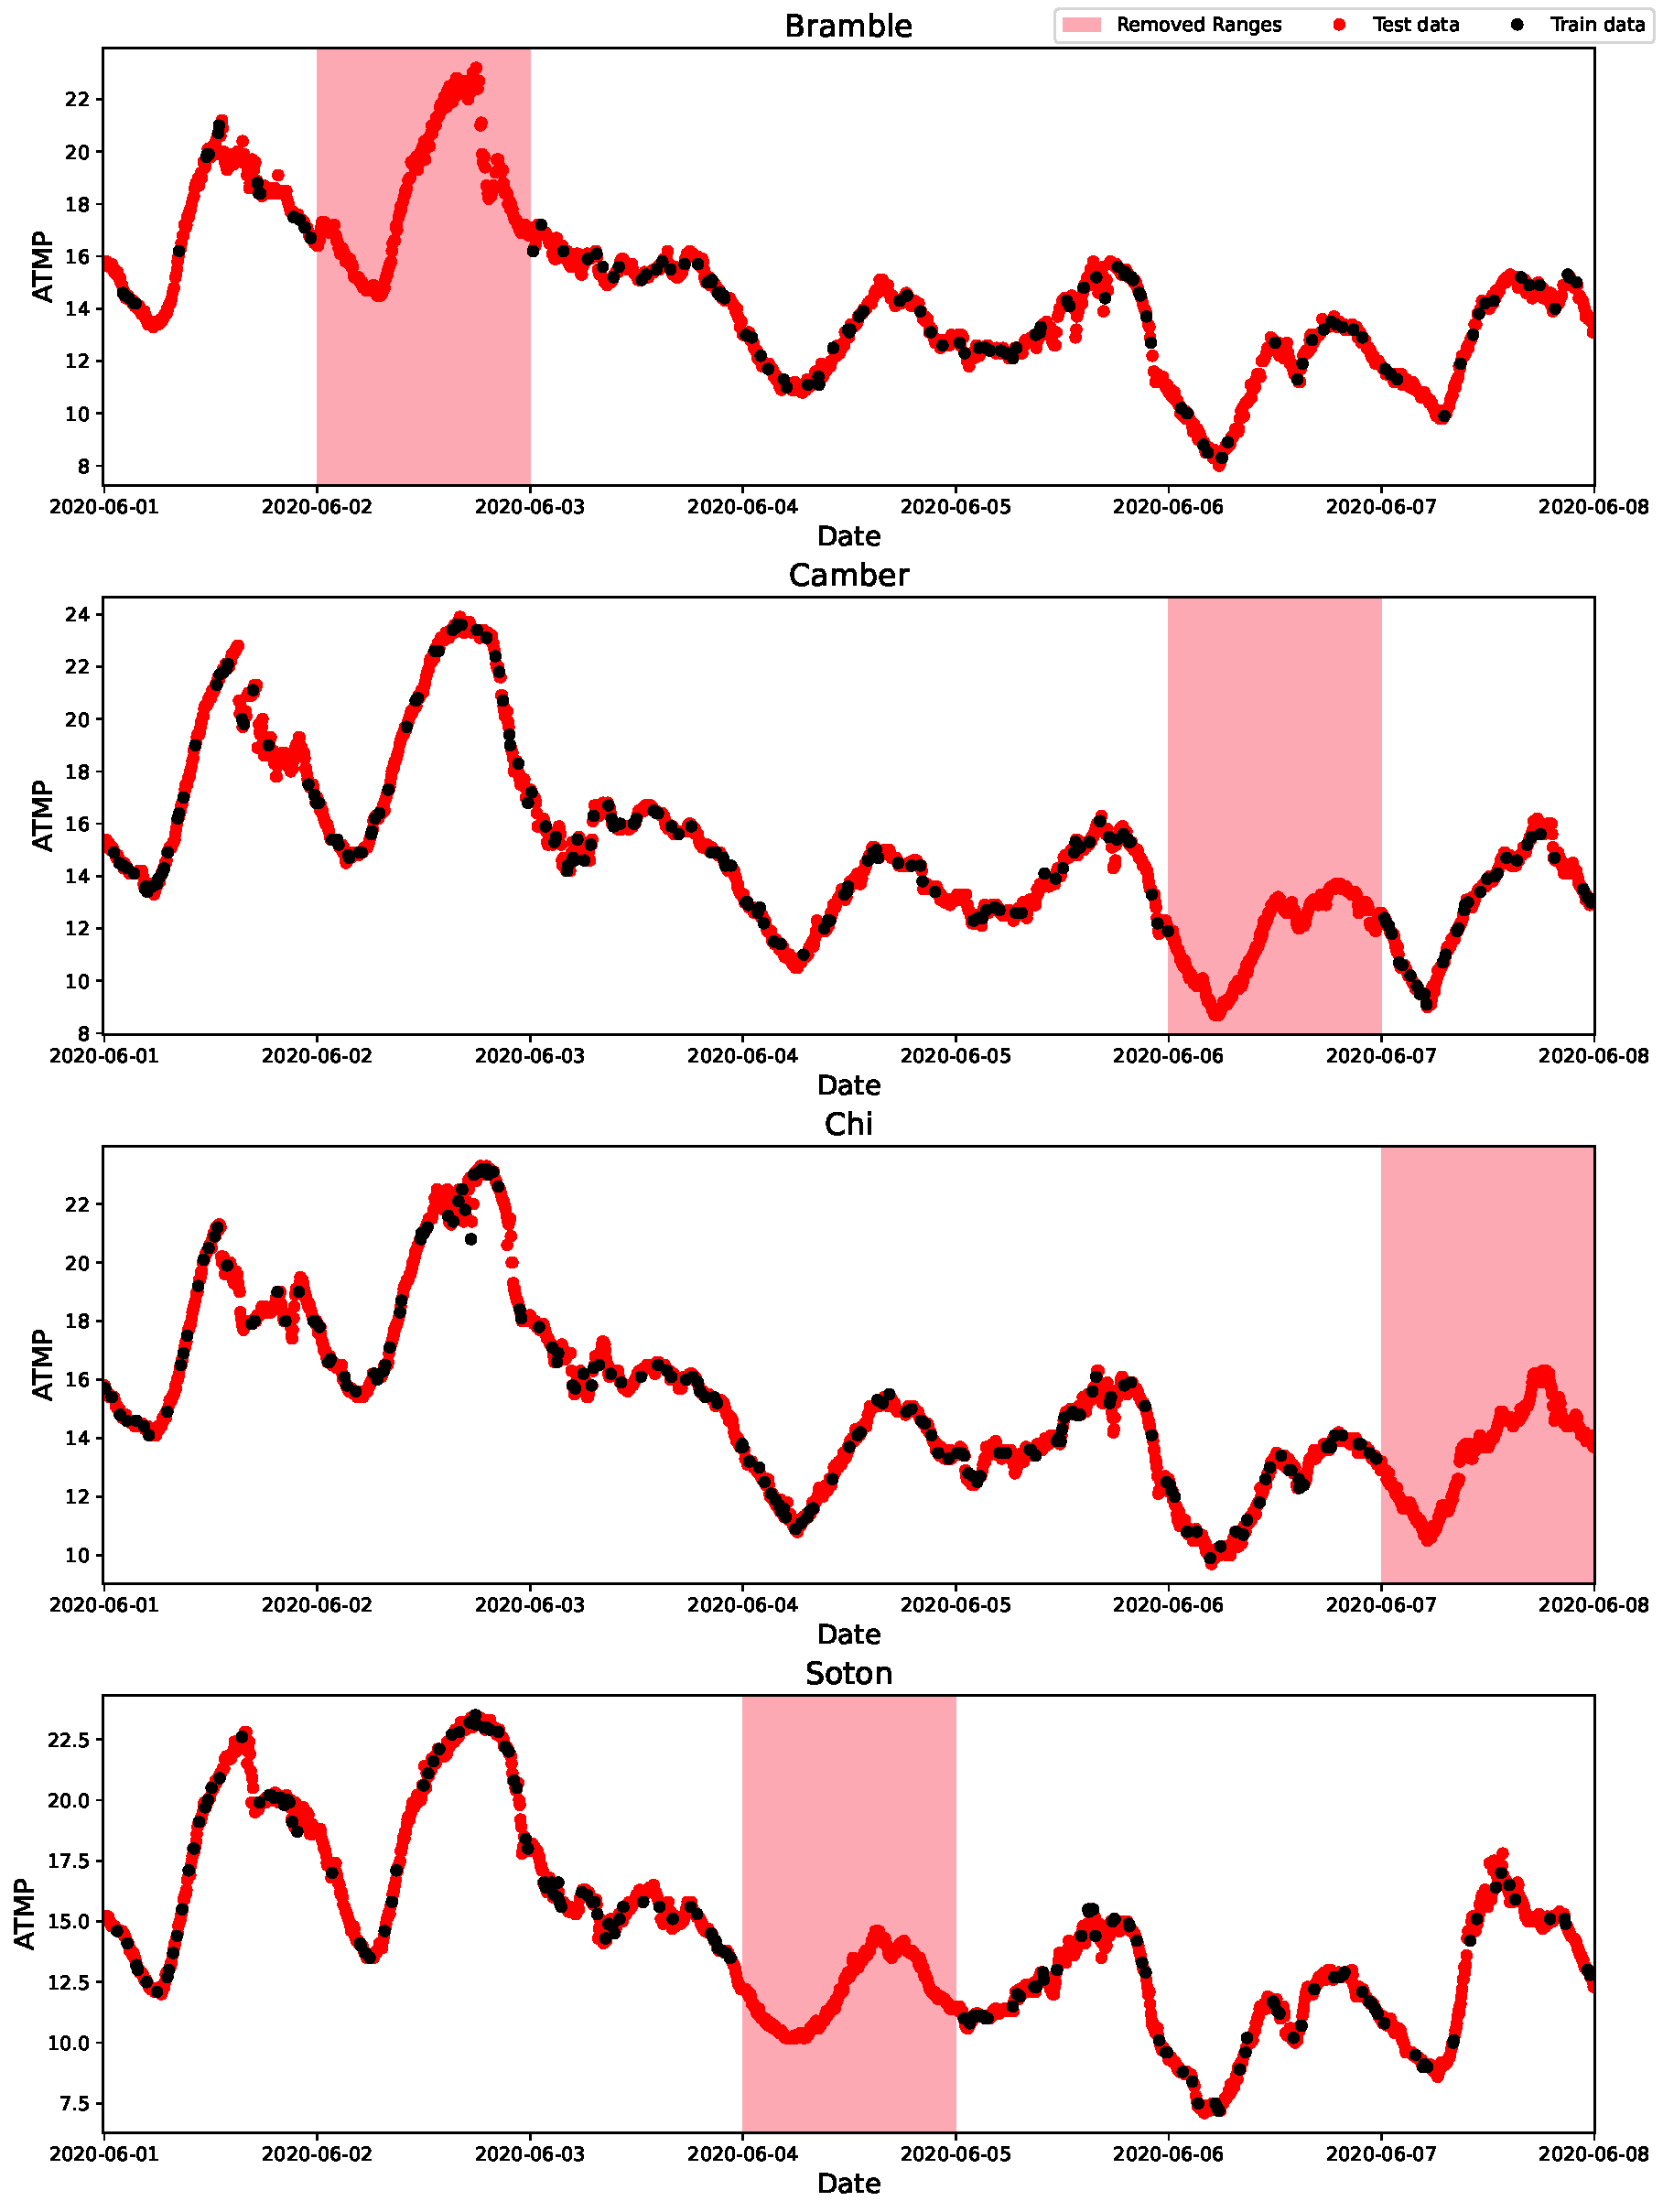
\includegraphics[scale=0.125]{ukcoast_atmp.pdf}}
      \subfigure{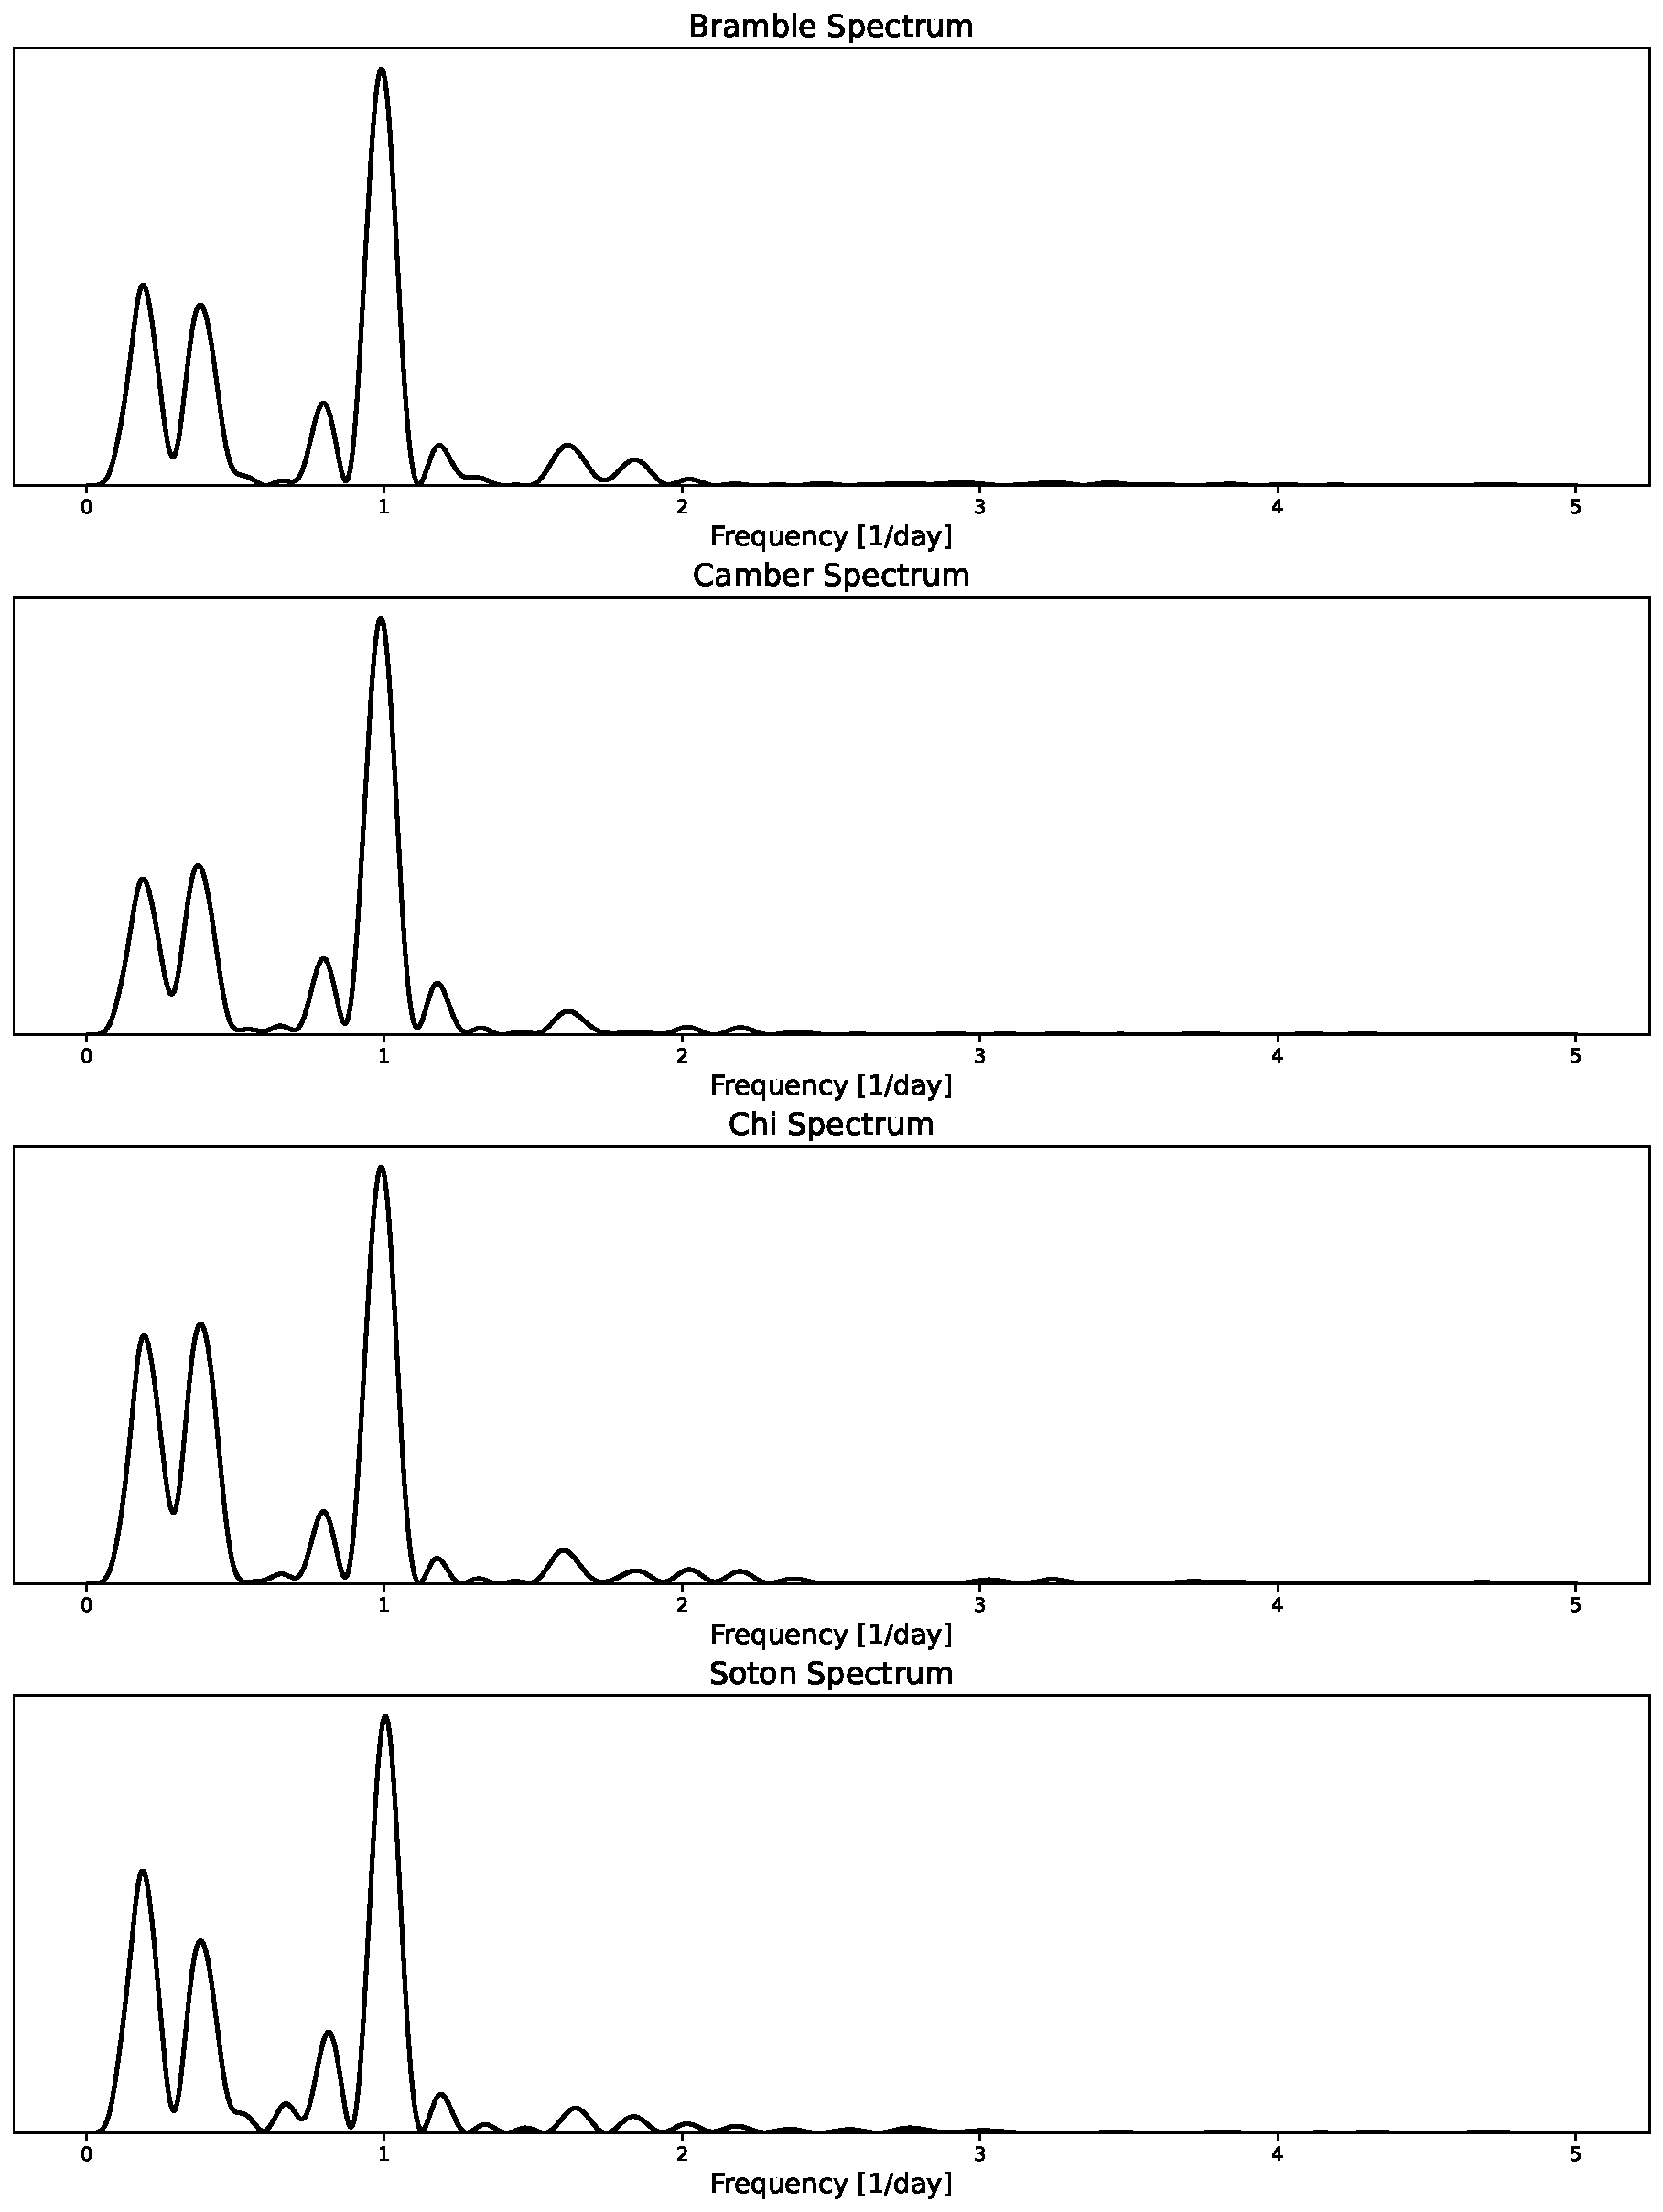
\includegraphics[scale=0.125]{ukcoast_atmp_spectrums.pdf}}
    \end{figure}
  \end{itemize}
\end{frame}

\begin{frame}{\subsecname}
  \begin{itemize}
    \item Série temporelle multivariée, $GP$ défini de $\mathcal{X} = \mathbb{R}^{+}$ (temps) vers $\mathcal{Y} = \mathbb{R}^{4}$ (stations)
    \pause
    \item Hypothèses: les stations sont corrélées, bruitées et périodiques
    %
    \item Deux niveaux de corrélation: \tored{intra}-station et \toblue{inter}-station
    \begin{equation*}
      \center
      \matrixx{K}(t, t^{\prime}) =
      \begin{pmatrix}
        \tored{k_{11}}(t, t^{\prime}) & \toblue{k_{12}}(t, t^{\prime}) & \toblue{k_{13}}(t, t^{\prime}) & \toblue{k_{14}}(t, t^{\prime}) \\
        \vdots                & \tored{k_{22}}(t, t^{\prime}) & \toblue{k_{23}}(t, t^{\prime}) & \toblue{k_{24}}(t, t^{\prime}) \\
        \vdots                & \vdots                & \ddots                & \vdots                        \\
        \toblue{k_{41}}(t, t^{\prime}) & \hdots                & \hdots                & \tored{k_{44}}(t, t^{\prime})
      \end{pmatrix}
    \end{equation*}
    %
    \item Chaque station doit être prédite avec par elle-même + les autres
  \end{itemize}
\end{frame}

\begin{frame}{\subsecname}
  \begin{itemize}
    \item Kernels "spectraux"\footnote{de la forme $k_{ij}(t, t^{\prime}) = 
    \alpha_{ij} e^{- \frac{(|t - t^{\prime}| + \theta_{ij})^2}{2 \Sigma_{ij}}}
    \cos((|t - t^{\prime}| + \theta_{ij})\mu_{ij} + \phi_{ij})$}\cite{Parra2017}: 
    fit les puissances spectrales pour estimer les périodicités intra/inter et filtrer le bruit (hautes fréquences)
    %
    \item Entraînement: $n=644$, test: $n=6845$, $84$ hyperparamètres (notebook dispo: détails optim etc.)
    %
    \item \dots
    %
    \item $1500$ itérations (1min 23s)
    %
    \item Comparaison avec le même kernel sans corrélation inter-station
  \end{itemize}
\end{frame}


\begin{frame}{\subsecname}
  \begin{table}[h]
    \centering
    \begin{subtable}%{0.1\linewidth}
      \centering
      \begin{tabular}{|l|c|c|c|}
        \hline
        & MAE & MAPE & RMSE \\
        \hline
        Bramble (NaN) & 2.10 & 10.37 & 2.79 \\
        Camber (NaN) & 1.58 & 13.82 & 1.74 \\
        Chi (forecast) & 1.76 & 12.53 & 2.01 \\
        Soton (NaN) & 1.68 & 15.00 & 2.13 \\
        \hline
      \end{tabular}
      \caption*{kernel \coloredemph{sans} corrélation inter-station}
    \end{subtable}%
    \begin{subtable}%{0.1\linewidth}
      \centering
      \begin{tabular}{|l|c|c|c|}
        \hline
        & MAE & MAPE & RMSE \\
        \hline
        Bramble & 0.65 & 3.44 & 0.89 \\
        Camber & 0.61 & 5.27 & 0.72 \\
        Chi & 0.61 & 4.72 & 0.71 \\
        Soton & 0.45 & 3.55 & 0.54 \\
        \hline
      \end{tabular}
      \caption*{kernel \coloredemph{avec} corrélation inter-station}
    \end{subtable}
    \caption{Erreurs de prédiction}
  \end{table}
\end{frame}

\begin{frame}{\subsecname}
  \begin{figure}
    \centering
      \subfigure{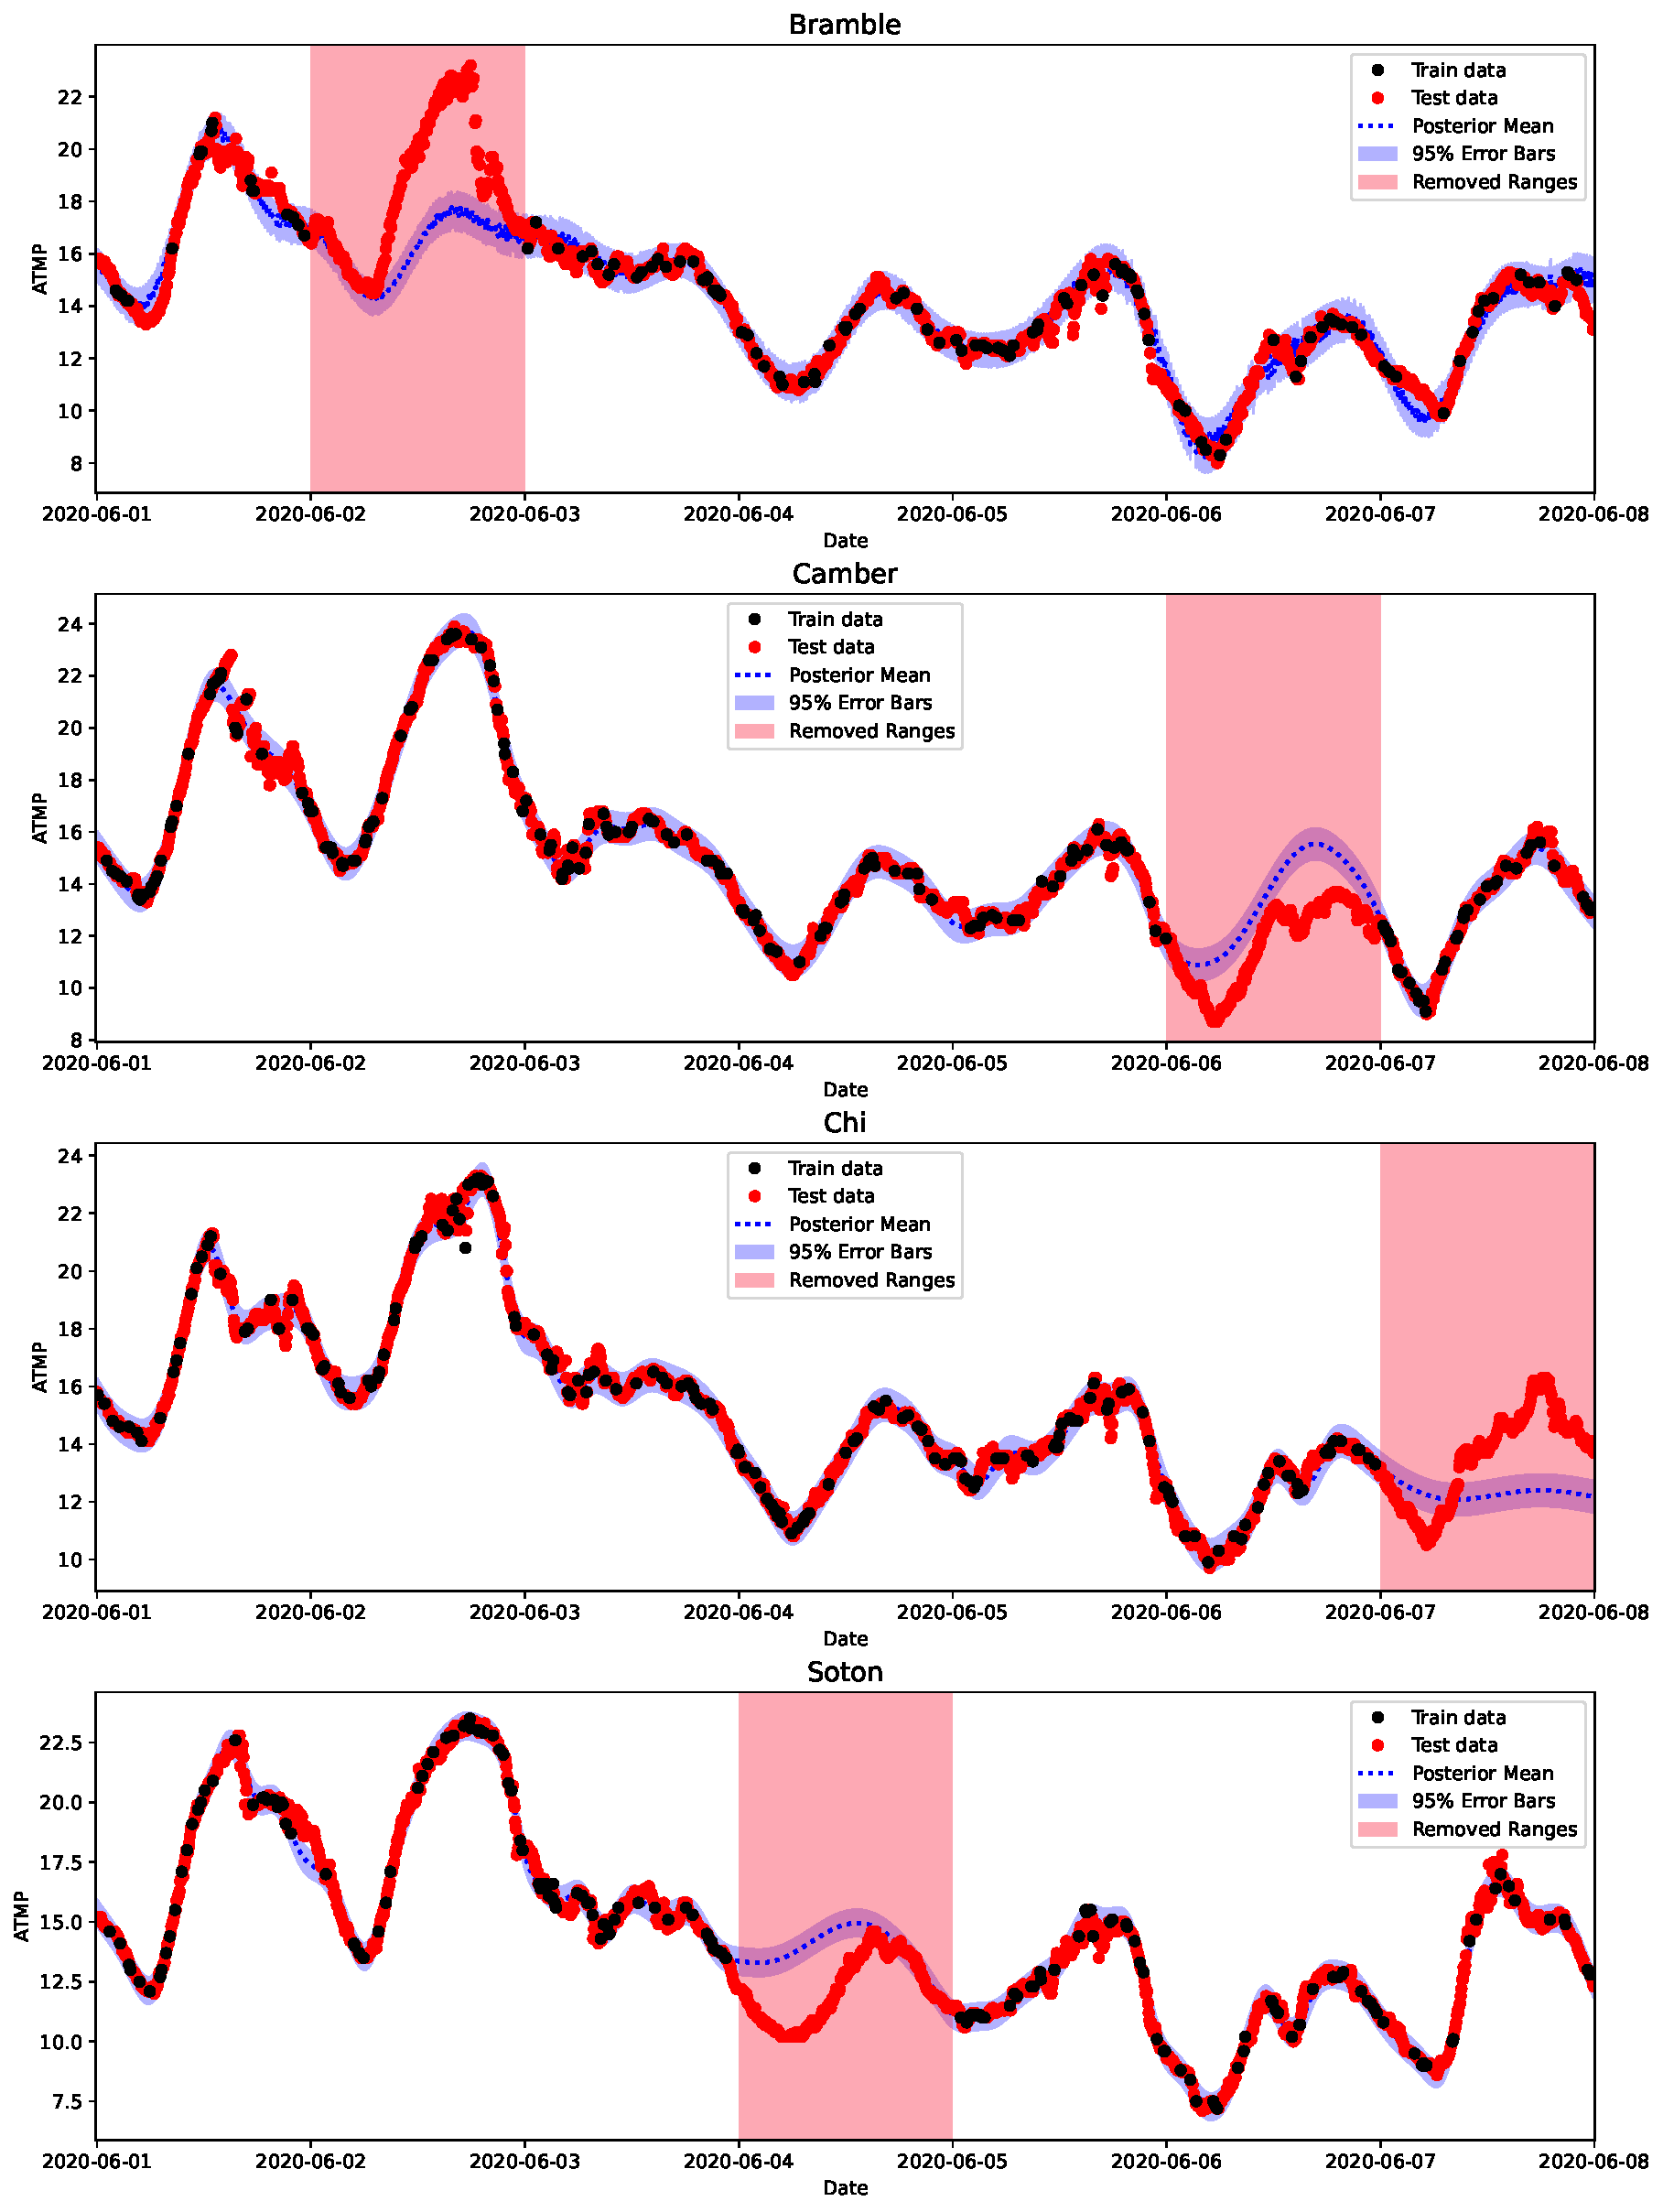
\includegraphics[scale=0.17]{ukcoast_pred_idsm.pdf}}
      \subfigure{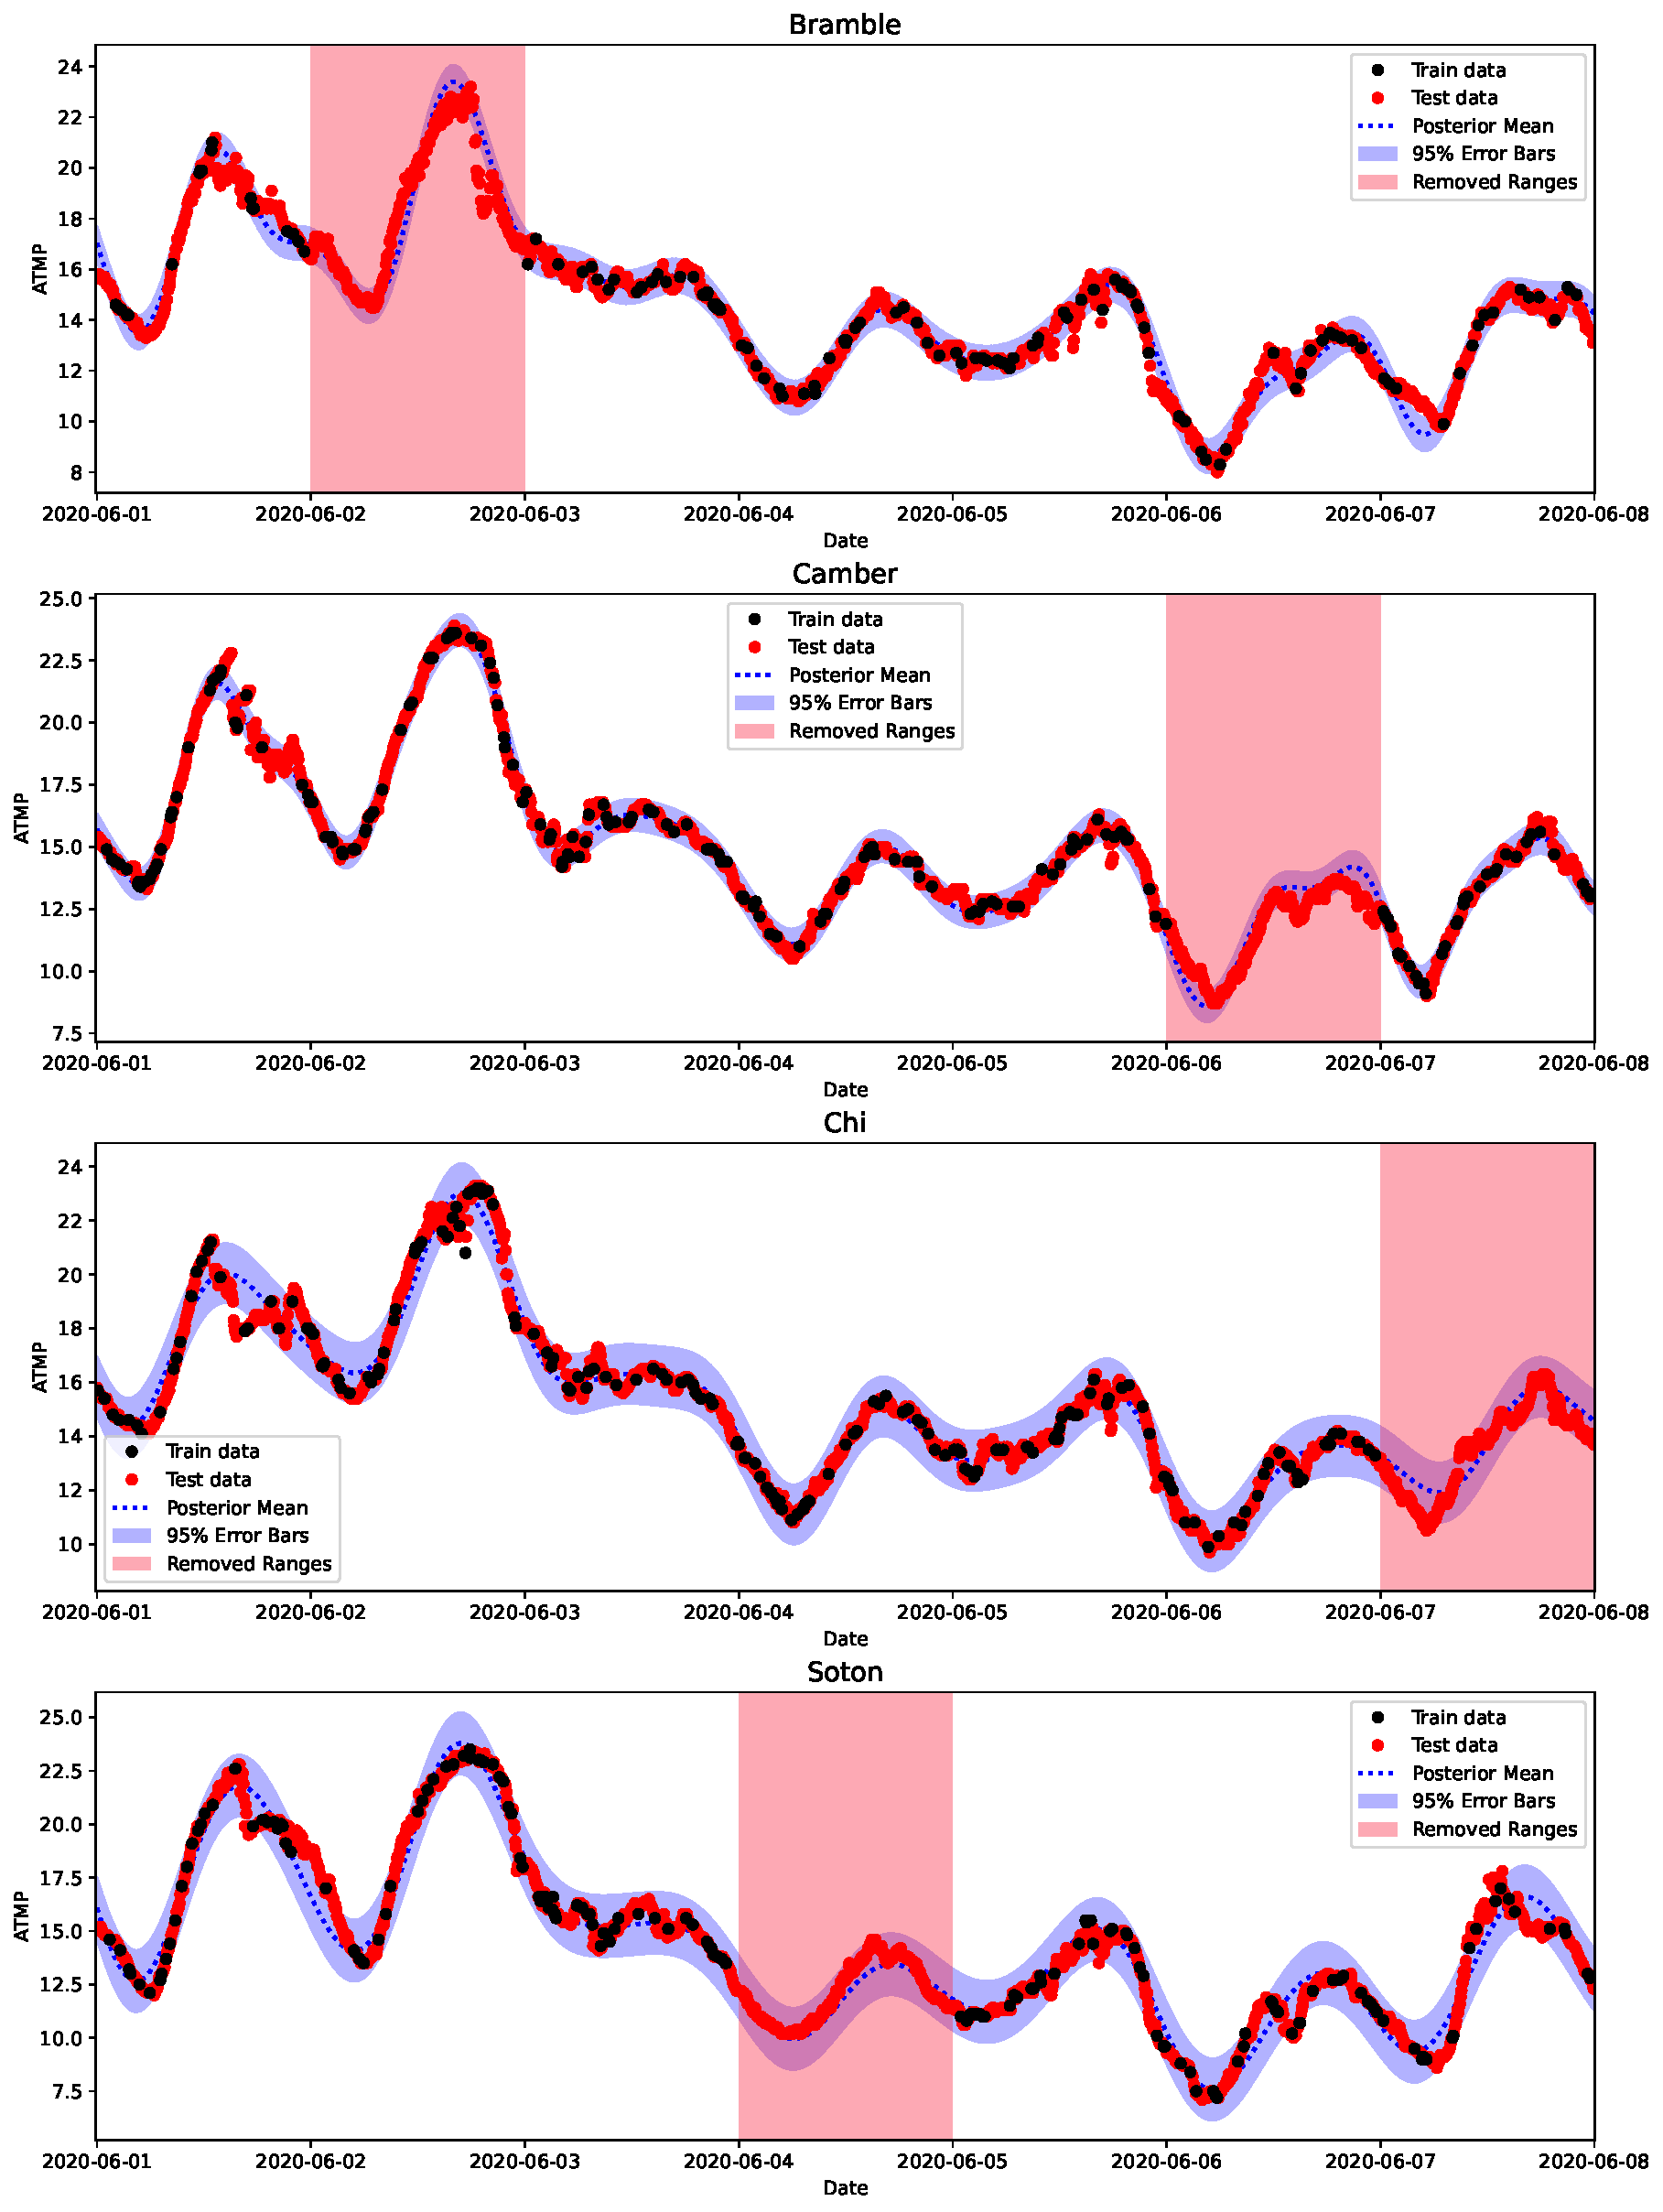
\includegraphics[scale=0.17]{ukcoast_pred_mosm.pdf}}
    \caption{Pédictions (rouge) sans (resp avec) corrélation inter-stations à gauche (resp droite)}
  \end{figure}
\end{frame}

\begin{frame}{\subsecname}
  \begin{itemize}
    \item Kernel appris par chaque modèle:
    \begin{figure}
      \centering
      \subfigure{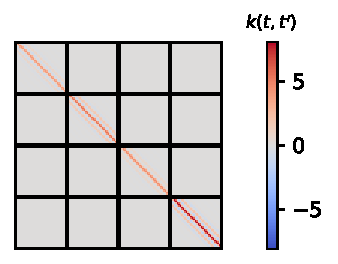
\includegraphics[scale=1]{ukcoast_crosskernel_idsm.pdf}}%
      \subfigure{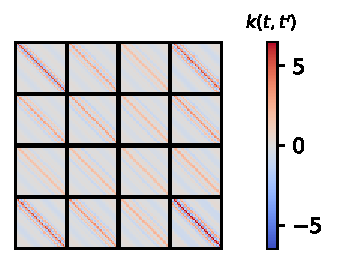
\includegraphics[scale=1]{ukcoast_crosskernel_mosm.pdf}}
      \caption{Kernel sans (resp avec) corrélation inter-stations à gauche (resp droite)}
    \end{figure}
    \pause
    \item Le modèle corrèle les prédictions de chaque station à court-terme
  \end{itemize}
\end{frame}

\begin{frame}{\subsecname}
  \begin{itemize}
    \item Prédictions probabilistes: 
    \pause
    \item Quelle est la probabilité qu'il fasse entre 13° et 14° à Bramble au 08/06/2020 à minuit ?
    %
    \item \toblue{Prédiction} du modèle: $59 \%$
    \pause
    \item A l'inverse: à la même date, quel intervalle à 90\% ?
    %
    \item \toblue{Prédiction} du modèle: $[14.2; 14.9]$° 
  \end{itemize}
\end{frame}

%========== Conclusion/opening ==================%
\section{Avantages / Limites des $GP$ naïfs}

\subsection{Avantages}
\begin{frame}{\subsecname}
  \begin{itemize}
    \item \coloredemph{Probabiliste}: génératif, fourni une confiance (aka incertitude)
    \pause
    \item \coloredemph{Bayésien}: "contrôle" des hypothèses (a priori)
    \pause
    \item \coloredemph{Non-paramétrique}: \toblue{prédiction} = \tored{data} $\times$ \topurple{hypothèse}
      \begin{enumerate}
        \item Paramètres du $GP$ (moyenne, covariance) = les/des \tored{données d'entraînement}, de taille infinie (non-bornée)
        \pause
        \item $+$ les \topurple{hyperparamètres} (ce qui règle l'hypothèse)
      \end{enumerate}
    \pause
    \item Le modèle prédictif n'est pas "réduit" à un ensemble \coloredemph{fini} de paramètres
    \pause
    \item Cadre naturel des données spatio/temporelles: échantillonnage irrégulier en temps ($\neq$ SARIMA) et espace, décomposition de la variabilité
    \pause
    \item Extensible à plus de dimensions d'entrée que le temps
  \end{itemize}
\end{frame}

\subsection{Limites}
\begin{frame}{\subsecname}
  Scalabilité:
  \begin{itemize}
    \item Bottleneck = inverser la matrice de covariance (kernel)
    \item La distribution prédictive $GP( m_{*}, k_{*, \theta} )$ est lourde à calculer ($n \gg 10^4$)
      \begin{itemize}
        \item \tored{Entraînement} (log-likelihood): calcul: $\mathcal{O}(n^3)$/itération. Mémoire: $\mathcal{O}(n^2)$
        \item \toblue{Prédiction} (inférence): calcul $\mathcal{O}(n^3)$ (une fois), 
      \end{itemize}
  \end{itemize}
\end{frame}

\begin{frame}{\subsecname}
  GP pour les données non-Gaussiennes ? \\ 
  \begin{itemize}
    \item<1-> Monde Gaussien: symmétrique, pas d'outliers, valeurs réelles
    \only<1-3>{
      \begin{equation*}
      \centering
      \only<2>{
        \overbrace{p(f_\theta | y, \vectorx{x}, x_0)}^{\toblue{posterior}}
        =
        \frac{
          \overbrace{p(y | \vectorx{x}, f_\theta)}^{\tored{likelihood}}
          \overbrace{p(f_\theta)}^{\topurple{prior = Gaussien}}
        }{
          \underbrace{p(y | \vectorx{x})}_{Gaussien}
        }
      }%
      %
      \only<3>{
        \overbrace{p(f_\theta | y, \vectorx{x}, x_0)}^{\toblue{posterior = Gaussien}}
        =
        \frac{
          \overbrace{p(y | \vectorx{x}, f_\theta)}^{\tored{likelihood = Gaussien}}
          \overbrace{p(f_\theta)}^{\topurple{prior = Gaussien}}
        }{
          \underbrace{p(y | \vectorx{x})}_{Gaussien}
        } 
        = GP(m_{*}, k_{*, \theta})
      }%
      \end{equation*}%
    }%
  \end{itemize}
\end{frame}

\begin{frame}{\subsecname}
  GP pour les données non-Gaussiennes ? \\ 
  \begin{itemize}
    \item<1->  Monde\underline{s} \coloredemph{non-Gaussiens}: 
    valeurs positives (durées, pluviométrie), comptage (nb d'accidents), valeurs extrèmes (rendements financiers), taux, catégorielles, etc.%
    %
    \\
    \only<1>{
      \begin{figure}
        \centering
        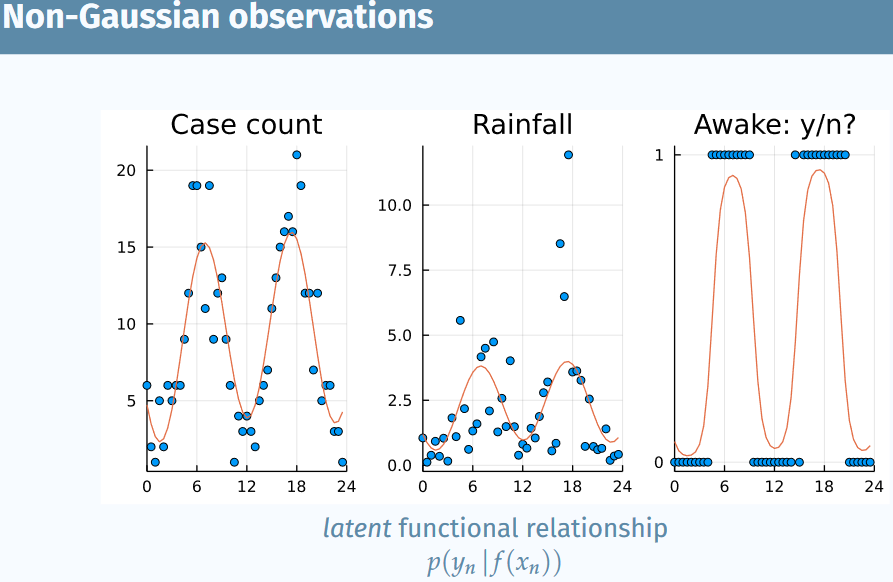
\includegraphics[scale=0.3]{non-guassian_ll.PNG}
        \caption*{Source: \href{https://gpss.cc/gpss22/slides/STJohn.pdf}{Gaussian Process Summer School 22'}}
      \end{figure}
    }
    \item<2-> Principe: transformer $\mathbb{E}(y)$ (espace latent) puis faire une hypothèse de GP sur la résultante.
    Prédiction en opération inverse.
    \item<3-> Exempe (classification): modéliser $\text{inv-logit} [ p(y=\text{Awake}) ]$ avec un $GP$
    \item<4-> Conséquence:%
    \only<5>{%
      \begin{equation*}
        \overbrace{p(f_\theta | y, \vectorx{x}, x_0)}^{\toblue{posterior = non-Gaussien}}
        =
        \frac{
          \overbrace{p(y | \vectorx{x}, f_\theta)}^{\tored{likelihood = non-Gaussien}}
          \overbrace{p(f_\theta)}^{\topurple{prior = Gaussien}}
        }{
          \underbrace{p(y | \vectorx{x})}_{non-Gaussien}
        } 
        = \xcancel{GP(m_{*}, k_{*, \theta})}
      \end{equation*}
    }%
  \end{itemize}
\end{frame}

\subsection{Remèdes}
\begin{frame}{\subsecname}
  $GP( m_{*}, k_{*, \theta} )$ est incalculable analytiquement ou trop coûteuse,
  \begin{itemize}
    \item Méthodes variationnelles: \cite{Bruinsma2020,Hensman2015}
    \item $GP( m_{*}, k_{*, \theta} )$ est \coloredemph{approximée} par une distribution "variationnelle" $q_{\psi}$, plus simple à apprendre
    \pause
    \item (hyper-) paramètres appris par minimisation d'une "différence"\footnote{Ex: divergence KL.}  entre $q_{\psi}$ et $GP( m_{*}, k_{*, \theta} )$
    \pause
    \item Le modèle d'inférence est donc appris en résolvant un problème d'\coloredemph{optimisation}: gradient stochastique, differentiation automatique (PyTorch, Tensorflow, JAX), etc.
  \end{itemize}
\end{frame}

\begin{frame}{\subsecname}
  Méthodes d'\coloredemph{échantillonnage} (MCMC, importance sampling, MH, etc): \cite{Rasmussen2006}
  \begin{itemize}
    \item Principe: remplacer $GP( m_{*}, k_{*, \theta} )$ par un échantillonneur peu coutêux
    \pause
    \item $m_{*}, k_{*, \theta}$ restent inconnus et sont estimés en échantillonnant (beaucoup) puis en moyennant (loi forte des grands nombres)
    % \item $GP( m_{*}, k_{*, \theta} ) = p(f_{*, \theta}|\tored{y, x}) = \int p(f_{*, \theta} | f_{\theta}) p(f_{\theta} | y) df$
  \end{itemize}
  \pause
  Méthode de \coloredemph{Kalman} ("State-space" model): \cite{Solin2014,Titsias2024}
  \begin{itemize}
    \item (uniquement pour les données temporelles)
    \pause
    \item Réécriture du $GP$ en équation différentielle stochastique
    \pause
    \item Apprentissage par l'algorithme de Kalman: $\xcancel{\mathcal{O}(n^3)}$, calcul $\mathcal{O}(n)$
    \pause
    \item La réecriture dépend du kernel: nécessite un kernel "pas trop compliqué" (état de recherche)
  \end{itemize}
\end{frame}

\begin{frame}
  Merci pour votre attention.
  \\
  Questions ?
\end{frame}

%
%======== References frame =========%
\begin{frame}[allowframebreaks]{Références}
  % \bibliographystyle{plain}
  \printbibliography
\end{frame}
\end{document}